%%%%%%%%%%%%%%%%%%%%%%%%%%%%%%%%%%%%%%%%%%  不使用 authblk 包制作标题  %%%%%%%%%%%%%%%%%%%%%%%%%%%%%%%%%%%%%%%%%%%%%%
%-------------------------------PPT Title-------------------------------------
\title{{\rm LAMMPS}算例举要}
%-----------------------------------------------------------------------------
%----------------------------Author & Date------------------------------------

%\author[\textrm{Jun\_Jiang}]{姜\;\;骏\inst{}} %[]{} (optional, use only with lots of authors)
%% - Give the names in the same order as the appear in the paper.
%% - Use the \inst{?} command only if the authors have different
%%   affiliation.
\institute[BCC]{\inst{}%
%\institute[Gain~Strong]{\inst{}%
\vskip -20pt 北京市计算中心~云平台事业部~~姜骏}
%\vskip -20pt {\large 格致斯创~科技}}
\date[\today] % (optional, should be abbreviation of conference name)
{%	{\fontsize{6.2pt}{4.2pt}\selectfont{\textcolor{blue}{E-mail:~}\url{jiangjun@bcc.ac.cn}}}
\vskip 45 pt {\fontsize{8.2pt}{6.2pt}\selectfont{%清华大学\;\;物理系% 报告地点
	\vskip 5 pt \textrm{2023.11.23-24}}}
}

%% - Either use conference name or its abbreviation
%% - Not really information to the audience, more for people (including
%%   yourself) who are reading the slides onlin%%   yourself) who are reading the slides onlin%%   yourself) who are reading the slides onlineee
%%%%%%%%%%%%%%%%%%%%%%%%%%%%%%%%%%%%%%%%%%%%%%%%%%%%%%%%%%%%%%%%%%%%%%%%%%%%%%%%%%%%%%%%%%%%%%%%%%%%%%%%%%%%%%%%%%%%%

\subject{}
% This is only inserted into the PDF information catalog. Can be left
% out.
%\maketitle
\frame
{
%	\frametitle{\fontsize{9.5pt}{5.2pt}\selectfont{\textcolor{orange}{“高通量并发式材料计算算法与软件”年度检查}}}
\titlepage
}
%-----------------------------------------------------------------------------

%------------------------------------------------------------------------------列出全文 outline ---------------------------------------------------------------------------------
\section{基本计算}\label{Sec:General}
%真空中的孤立原子的基态能量是\textrm{VASP}中最简单的算例,通过学习金属\textrm{Pt}原子基态能量的计算,可以掌握典型的\textrm{VASP}的主体流程\footnote{在所有计算之前,请确认\textrm{VASP}软件已经正确安装。},了解体系基态能量最小化的基本算法,并熟悉基本的输入/输出文件的内容。此外,还可以了解如何在已完成计算的基础上,进行计算精度提升或完成后续计算等一系列处理方式。
%\subsection{输入文件}
\frame
{
	\frametitle{\textrm{LAMMPS}一般计算流程}
\begin{figure}[h!]
\centering
\vskip -5pt
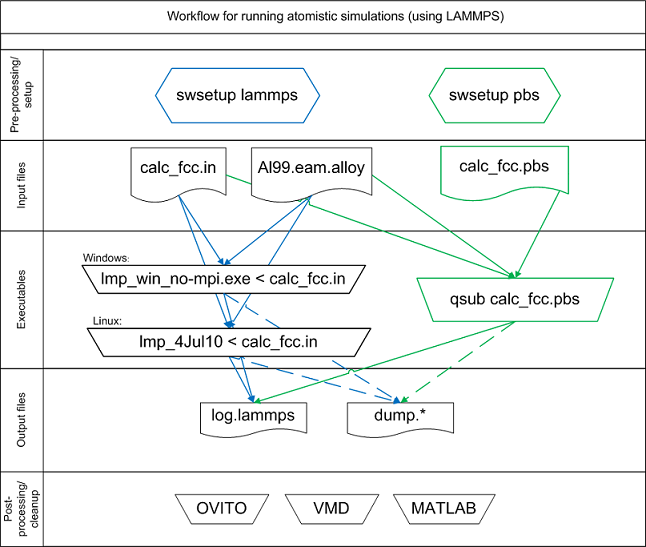
\includegraphics[height=2.50in,width=3.0in, viewport=0 0 646 547,clip]{Lammps_workflow.png}
\caption{\fontsize{6.2pt}{5.2pt}\selectfont{\textrm{The general workflow for running molecular dynamics simulations using LAMMPS.}}}%(与文献\cite{EPJB33-47_2003}图1对比)
\label{General_Workflow}
\end{figure}
}

\subsection{能量最小化}
\frame
{
	\frametitle{\textrm{LAMMPS}的输入参数说明}
	{\fontsize{7.5pt}{6.0pt}\selectfont{
%\verbatiminput{Figures/Lammps_in_lj.txt} %为保险:~选用文件名绝对路径
\verbatiminput{Figures/Lammps_tutorial-01-in_01.txt} %为保险:~选用文件名绝对路径
}
\begin{itemize}
	\item \textcolor{cyan}{\textit{\#}}~开头的部分表示注释,\textrm{LAMMPS}不作任何处理
\end{itemize}
}
\vskip 5pt
%\textrm{LAMMPS}模拟的初始化
{\fontsize{7.5pt}{6.0pt}\selectfont{
%\verbatiminput{Figures/Lammps_in_lj.txt} %为保险:~选用文件名绝对路径
\verbatiminput{Figures/Lammps_tutorial-01-in_02-1.txt} %为保险:~选用文件名绝对路径
\begin{itemize}
	\item \textcolor{cyan}{\textit{clear}}:~清除全部内存信息
	\item \textcolor{cyan}{\textit{unit}}:~设定模拟的单位~ (\textcolor{blue}{\textrm{metal}}~表示选择\textrm{\AA}和\textrm{eV}为单位)
	\item \textcolor{cyan}{\textit{dimension}}:~设定模拟维度~:~\textcolor{blue}{\textrm{3}}~表示三维模拟
	\item \textcolor{cyan}{\textit{boundary}}~\textcolor{blue}{\textrm{p~p~p}}:~表示在$x$-,$y$-,$z$-方向采用周期性边界条件
		\begin{itemize}
{\fontsize{6.2pt}{5.0pt}\selectfont{
			\item \textrm{p}:~周期性边界条件\textrm{(periodic)}
			\item \textrm{f}:~非周期性固定边界条件\textrm{(fixed)}
			\item \textrm{s}:~非周期性包覆边界条件\textrm{(shrink-wrapped)}
			\item \textrm{m}:~非周期性包覆最小值边界条件\textrm{(minimum value)}}}
		\end{itemize}
\end{itemize}
}}
}

\frame
{
	\frametitle{\textrm{LAMMPS}的输入参数说明}
	{\fontsize{7.5pt}{6.0pt}\selectfont{
\verbatiminput{Figures/Lammps_tutorial-01-in_02-2.txt} %为保险:~选用文件名绝对路径
\begin{itemize}
	\item \textcolor{cyan}{\textit{atom\_style}}:~设置计算粒子类型~:~\textcolor{blue}{\textrm{atomic}}表示普通原子类型
		\vskip 4pt
		在反应力场计算中,\textcolor{cyan}{\textit{atom\_style}}选用\textcolor{blue}{\textrm{charge}},而\textcolor{cyan}{\textit{units}}选用\textcolor{blue}{\textrm{full}},即反应力场中需要考虑电荷平衡问题
	\item \textcolor{cyan}{\textit{atom\_modify}}:~\textcolor{blue}{\textrm{map~array}}:~表示设置和定义某些存储原子的属性
	\vskip 4pt
	\textcolor{purple}{语法规则}:~\textcolor{cyan}{\textit{atom\_modify}}:~\textcolor{blue}{\textrm{keyword~value}}
	\vskip 3pt
	\textrm{keyword}:~\textrm{\textcolor{blue}{id}~/~\textcolor{blue}{map}~/~\textcolor{blue}{first}}
		\begin{itemize}
{\fontsize{6.2pt}{5.0pt}\selectfont{
\item \textcolor{blue}{\textrm{id~value}}=\textrm{yes~or~no}:~设置是否储存每一个原子的\textrm{ID}(序号) 默认为~\textrm{yes}
\item \textcolor{blue}{\textrm{map~value}}=\textrm{yes~or~array~or~hash}:~设置如何在需要时具有特定\textrm{ID}的原子被发现(\textrm{array}~比\textrm{hash}~快)
\item \textcolor{blue}{\textrm{first~value}}=\textrm{group~ID}:~\textrm{group~ID}~原子首先出现在内部原子列表中的组}}
		\end{itemize}
		\end{itemize}
	}}
}

\frame
{
	\frametitle{\textrm{LAMMPS}的输入参数说明}
	{\fontsize{7.5pt}{6.0pt}\selectfont{
%\verbatiminput{Figures/Lammps_in_lj.txt} %为保险:~选用文件名绝对路径
\verbatiminput{Figures/Lammps_tutorial-01-in_03.txt} %为保险:~选用文件名绝对路径
}
\begin{itemize}
	\item \textcolor{cyan}{\textit{lattice}}:~设定晶格信息~(可选择的晶格类型有\textrm{sc, fcc, bcc, hcp, diamond}等)、\\
		晶格常数(数值\textrm{4})、晶格矢量方向等
	\item \textcolor{cyan}{\textit{region}}:~设定模拟的原胞,此处设定模拟的名为\textcolor{blue}{\textrm{box}}的\textrm{block}(可以理解为原胞)采用晶格单位,并要求\textrm{box}每个方向的大小取为一个晶格常数
	\item \textcolor{cyan}{\textit{create\_box}}:~使用\textcolor{cyan}{\textit{region}}确定的参数构建模拟的\textrm{box},数量为\textcolor{red}{1个}
	\item \textcolor{cyan}{\textit{replicate}}:~设定每个方向上重复的元胞数目
\end{itemize}
}
}

\frame
{
	\frametitle{\textrm{LAMMPS}的输入参数说明}
%\textrm{LAMMPS}模拟的初始化
{\fontsize{7.5pt}{6.0pt}\selectfont{
%\verbatiminput{Figures/Lammps_in_lj.txt} %为保险:~选用文件名绝对路径
\verbatiminput{Figures/Lammps_tutorial-01-in_04.txt} %为保险:~选用文件名绝对路径
}
\begin{itemize}
	\item \textcolor{cyan}{\textit{pair\_style}}:~设定原子间相互作用(力场)类型,此处势函数的形式为~\textcolor{blue}{\textrm{eam/alloy}}
	\item \textcolor{cyan}{\textit{pair\_coeff}}~\textcolor{blue}{\textrm{$\ast$~$\ast$~Al99.eam.alloy~Al}}:~设定相互作用势(力场)的系数\\
		{\fontsize{6.2pt}{5.2pt}\selectfont{\textcolor{magenta}{势函数(力场)的扩展名提示的是使用相互作用的类型}~\textrm{(eam.alloy~=~eam/alloy)}}}
	\item \textcolor{cyan}{\textit{neighbor}}:~设置表面距离
	\item \textcolor{cyan}{\textit{neigh\_modify}}:~设置原子运动
\end{itemize}
}
}

\frame
{
	\frametitle{\textrm{LAMMPS}的输入参数说明}
	{\fontsize{7.5pt}{6.0pt}\selectfont{
%\verbatiminput{Figures/Lammps_in_lj.txt} %为保险:~选用文件名绝对路径
\verbatiminput{Figures/Lammps_tutorial-01-in_05.txt} %为保险:~选用文件名绝对路径
}
\begin{itemize}
	\item \textcolor{cyan}{\textit{compute}}:~定义计算变量:\\
		\begin{enumerate}
{\fontsize{7.5pt}{5.0pt}\selectfont{
\item \textcolor{purple}{变量\textrm{eng}}:~定义为平均每个原子的势能,并且存储在\textrm{ID:~eng}中
\item \textcolor{purple}{变量\textrm{eatom}}:~定义为求和全部\textcolor{purple}{变量\textrm{eng}}的值:~\textcolor{blue}{\textrm{reduce}}~表示减(负),对\textrm{eng}求和并存储在\textrm{ID:~eatoms}中}}
		\end{enumerate}
\end{itemize}
}
}

\frame
{
	\frametitle{\textrm{LAMMPS}的输入参数说明}
%\vskip 5pt
%\textrm{LAMMPS}模拟的初始化
{\fontsize{7.5pt}{6.0pt}\selectfont{
%\verbatiminput{Figures/Lammps_in_lj.txt} %为保险:~选用文件名绝对路径
\verbatiminput{Figures/Lammps_tutorial-01-in_06.txt} %为保险:~选用文件名绝对路径
}
\begin{itemize}
	\item \textcolor{cyan}{\textit{reset\_timestep}}:~重新设定时间模拟步数\footnote{\fontsize{6.2pt}{5.2pt}\selectfont{\textrm{LAMMPS}模拟中,一般需要设置能量最小化、弛豫、数据采集等阶段,不同阶段模拟步数不同。默认情况下,模拟步数是从模拟开始到模拟结束一直累加计算的}}(此处归零:~\textcolor{blue}{\textrm{0}})
	\item \textcolor{cyan}{\textit{fix}}:~设定\textrm{box/relax},能量最小化过程中对模拟盒施外压,各向同性\textrm{(iso)}都弛豫到\textrm{0.0~Pa}:~\textcolor{blue}{\textrm{vmax}}:~正压压缩,负压膨胀
	\item \textcolor{cyan}{\textit{thermo}}:~每运行\textcolor{blue}{10}次在屏幕上输出一次运行结果
	\item \textcolor{cyan}{\textit{thermo\_style}}:~设定屏幕输出信息
	\item \textcolor{cyan}{\textit{min\_style}}:~设定优化算法(最小化算法),\textcolor{blue}{\textrm{cg}}~指定共轭梯度法
	\item \textcolor{cyan}{\textit{minimize}}:~设定开始最小化过程和最小化收敛精度和最大迭代次数:\\
		其中1,3项为能量最小化,2,4项为能量梯度(力)\\
		(原胞弛豫的模拟由晶格常数为\textrm{4\AA}到\textrm{4.05\AA})
\end{itemize}
}
}

\frame
{
	\frametitle{\textrm{LAMMPS}的输入参数说明}
	{\fontsize{7.5pt}{6.0pt}\selectfont{
%\verbatiminput{Figures/Lammps_in_lj.txt} %为保险:~选用文件名绝对路径
\verbatiminput{Figures/Lammps_tutorial-01-in_07.txt} %为保险:~选用文件名绝对路径
}
\begin{itemize}
	\item \textcolor{cyan}{\textit{natoms}}:~变量定义所有原子数
	\item \textcolor{cyan}{\textit{teng}}:~变量定义总的势能:~\textcolor{blue}{\textrm{teng=eatoms}}
	\item \textcolor{cyan}{\textit{length}}:~变量定义模拟原胞长度:~\textcolor{blue}{\textrm{length=lx}}(模拟盒$x$方向为例)
	\item \textcolor{cyan}{\textit{ecoh}}:~变量定义内聚能:~\textcolor{blue}{\textrm{ecoh=v\_teng/v\_natoms}}\footnote{\fontsize{6.2pt}{5.2pt}\selectfont{同一语句中出现多个变量引用时用\textrm{\textcolor{red}{v}\_variable}表示}}
\end{itemize}}
%\textrm{LAMMPS}模拟的初始化
{\fontsize{7.5pt}{6.0pt}\selectfont{
%\verbatiminput{Figures/Lammps_in_lj.txt} %为保险:~选用文件名绝对路径
\verbatiminput{Figures/Lammps_tutorial-01-in_08.txt} %为保险:~选用文件名绝对路径
}
\begin{itemize}
	\item 设定屏幕输出和\textrm{log}文件的输出变量
	\item \textcolor{red}{\$\{\}}表示定义变量的引用
\end{itemize}
}
}

%\frame[allowframebreaks]
%{
%	\frametitle{\textrm{LAMMPS}的输入文件}
%\fontsize{6.0pt}{5.0pt}\selectfont{
%%\verbatiminput{Figures/Lammps_in_lj.txt} %为保险:~选用文件名绝对路径
%\verbatiminput{Figures/Lammps_tutorial-01-Lammps-in.txt} %为保险:~选用文件名绝对路径
%}
%}
%
\frame
{
	\frametitle{\textrm{LAMMPS}的输出结果}
	\textrm{LAMMPS}执行命令:
	\vskip 5pt
	\textcolor{blue}{lmp}~\textcolor{magenta}{-in}~calc\_fcc.in
	\vskip 5pt
\begin{figure}[h!]
\centering
\vskip -5pt
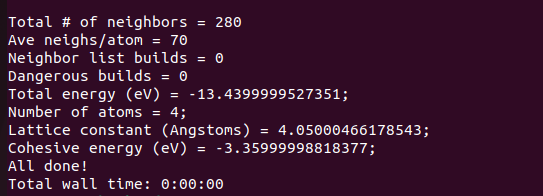
\includegraphics[height=1.50in,width=4.0in, viewport=0 0 543 196,clip]{Lammps_output.png}
\caption{\fontsize{6.2pt}{5.2pt}\selectfont{\textrm{The end of the logfile/screen output using LAMMPS.}}}%(与文献\cite{EPJB33-47_2003}图1对比)
\label{LAMMPS_output}
\end{figure}
}

\subsection{状态方程}
\frame[allowframebreaks]
{
	\frametitle{\textrm{LAMMPS}的输入文件}
	{\fontsize{6.0pt}{5.0pt}\selectfont{
%\verbatiminput{Figures/Lammps_in_lj.txt} %为保险:~选用文件名绝对路径
\verbatiminput{Figures/Lammps_tutorial-02-in.txt} %为保险:~选用文件名绝对路径
}}
\textrm{LAMMPS}执行命令~\textcolor{blue}{(指定变量)}:
	\vskip 5pt
	\textcolor{blue}{lmp}~\textcolor{magenta}{-in}~calc\_fcc.in~\textcolor{red}{-var~latconst~4}
}

\frame[allowframebreaks]
{
	\frametitle{\textrm{LAMMPS}的输入文件:~基于\textrm{Matlab}的执行}
	{\fontsize{6.0pt}{5.0pt}\selectfont{
%\verbatiminput{Figures/Lammps_in_lj.txt} %为保险:~选用文件名绝对路径
\verbatiminput{Figures/Lammps_tutorial-02-Lammps-in.txt} %为保险:~选用文件名绝对路径
}}
}

\frame[allowframebreaks]
{
	\frametitle{\textrm{LAMMPS}的输入文件:~基于\textrm{Matlab}的执行}
	{\fontsize{6.0pt}{5.0pt}\selectfont{
%\verbatiminput{Figures/Lammps_in_lj.txt} %为保险:~选用文件名绝对路径
\verbatiminput{Figures/Lammps_tutorial-02-Matlab-in.txt} %为保险:~选用文件名绝对路径
}}
}

\frame[allowframebreaks]
{
	\frametitle{\textrm{LAMMPS}的输入文件:~基于\textrm{Python}的执行}
	{\fontsize{6.0pt}{5.0pt}\selectfont{
%\verbatiminput{Figures/Lammps_in_lj.txt} %为保险:~选用文件名绝对路径
\verbatiminput{Figures/Lammps_tutorial-02-Python-in1.txt} %为保险:~选用文件名绝对路径
}}
}

\frame[allowframebreaks]
{
	\frametitle{\textrm{LAMMPS}的输入文件:~基于\textrm{Python}的执行}
	{\fontsize{6.0pt}{5.0pt}\selectfont{
%\verbatiminput{Figures/Lammps_in_lj.txt} %为保险:~选用文件名绝对路径
\verbatiminput{Figures/Lammps_tutorial-02-Python-in2.txt} %为保险:~选用文件名绝对路径
}}
}

\frame
{
	\frametitle{状态方程}
\begin{figure}[h!]
\centering
\vskip -5pt
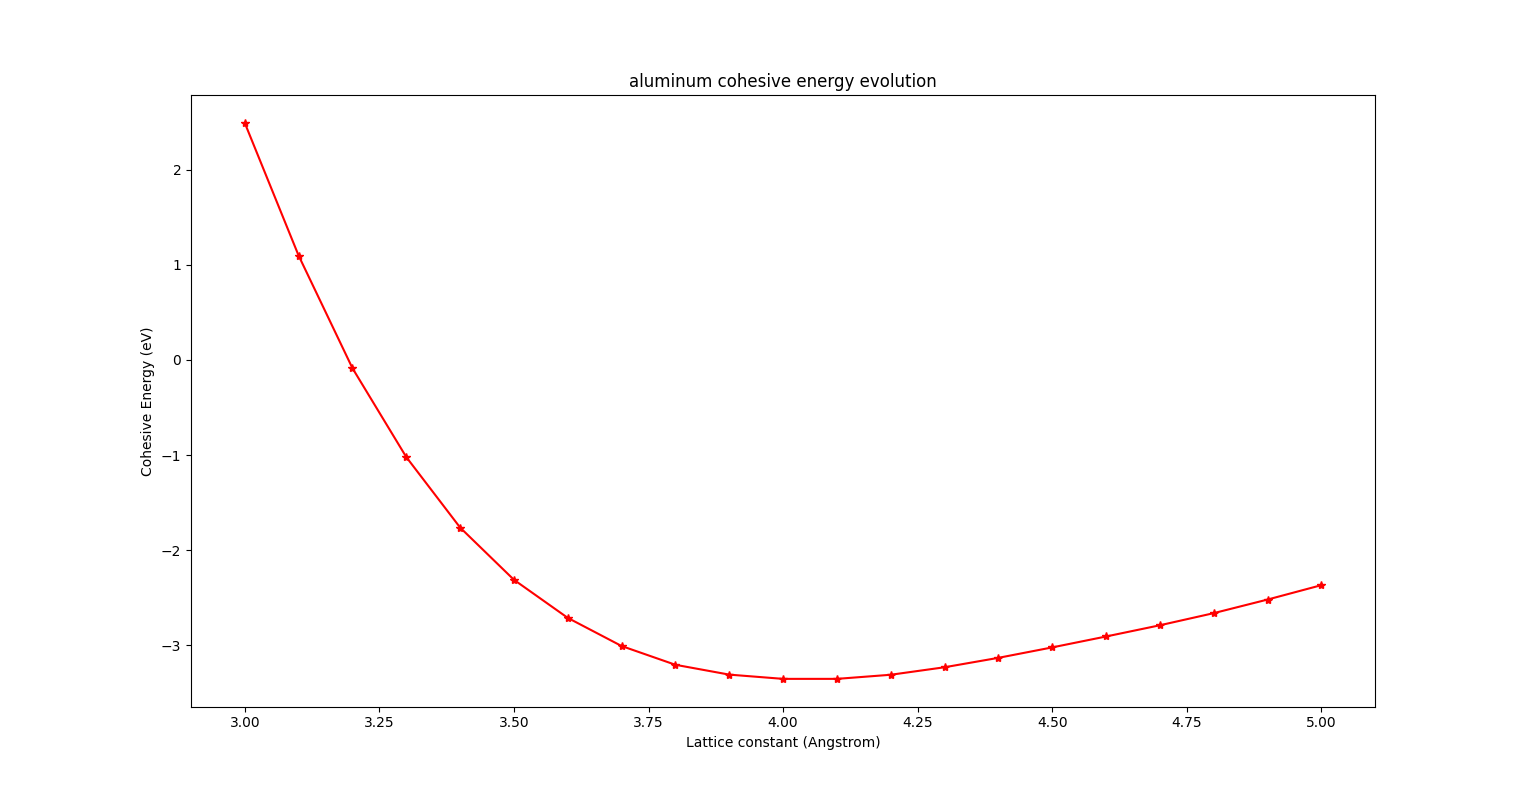
\includegraphics[height=2.50in,width=4.0in, viewport=0 0 1050 554,clip]{Lammps-EOS.png}
\caption{\fontsize{6.2pt}{5.2pt}\selectfont{\textrm{Aluminum cohesive energy evolution.}}}%(与文献\cite{EPJB33-47_2003}图1对比)
\label{LAMMPS_output-EOS}
\end{figure}
}

\subsection{拉伸与压力下的形变模拟}
\frame[allowframebreaks]
{
	\frametitle{\textrm{LAMMPS}的输入文件}
	{\fontsize{6.0pt}{5.0pt}\selectfont{
%\verbatiminput{Figures/Lammps_in_lj.txt} %为保险:~选用文件名绝对路径
\verbatiminput{Figures/Lammps_tutorial-03-Lammps-in.txt} %为保险:~选用文件名绝对路径
}}
}

\frame[allowframebreaks]
{
	\frametitle{\textrm{LAMMPS}的输入文件:~基于\textrm{Matlab}的执行}
	{\fontsize{6.0pt}{5.0pt}\selectfont{
%\verbatiminput{Figures/Lammps_in_lj.txt} %为保险:~选用文件名绝对路径
\verbatiminput{Figures/Lammps_tutorial-03-Matlab-in.txt} %为保险:~选用文件名绝对路径
}}
}

\frame[allowframebreaks]
{
	\frametitle{\textrm{LAMMPS}的输入文件:~基于\textrm{Python}的执行}
	{\fontsize{6.0pt}{5.0pt}\selectfont{
%\verbatiminput{Figures/Lammps_in_lj.txt} %为保险:~选用文件名绝对路径
\verbatiminput{Figures/Lammps_tutorial-03-Python-in.txt} %为保险:~选用文件名绝对路径
}}
}

\frame
{
	\frametitle{应力-应变曲线}
\begin{figure}[h!]
\centering
\vskip -5pt
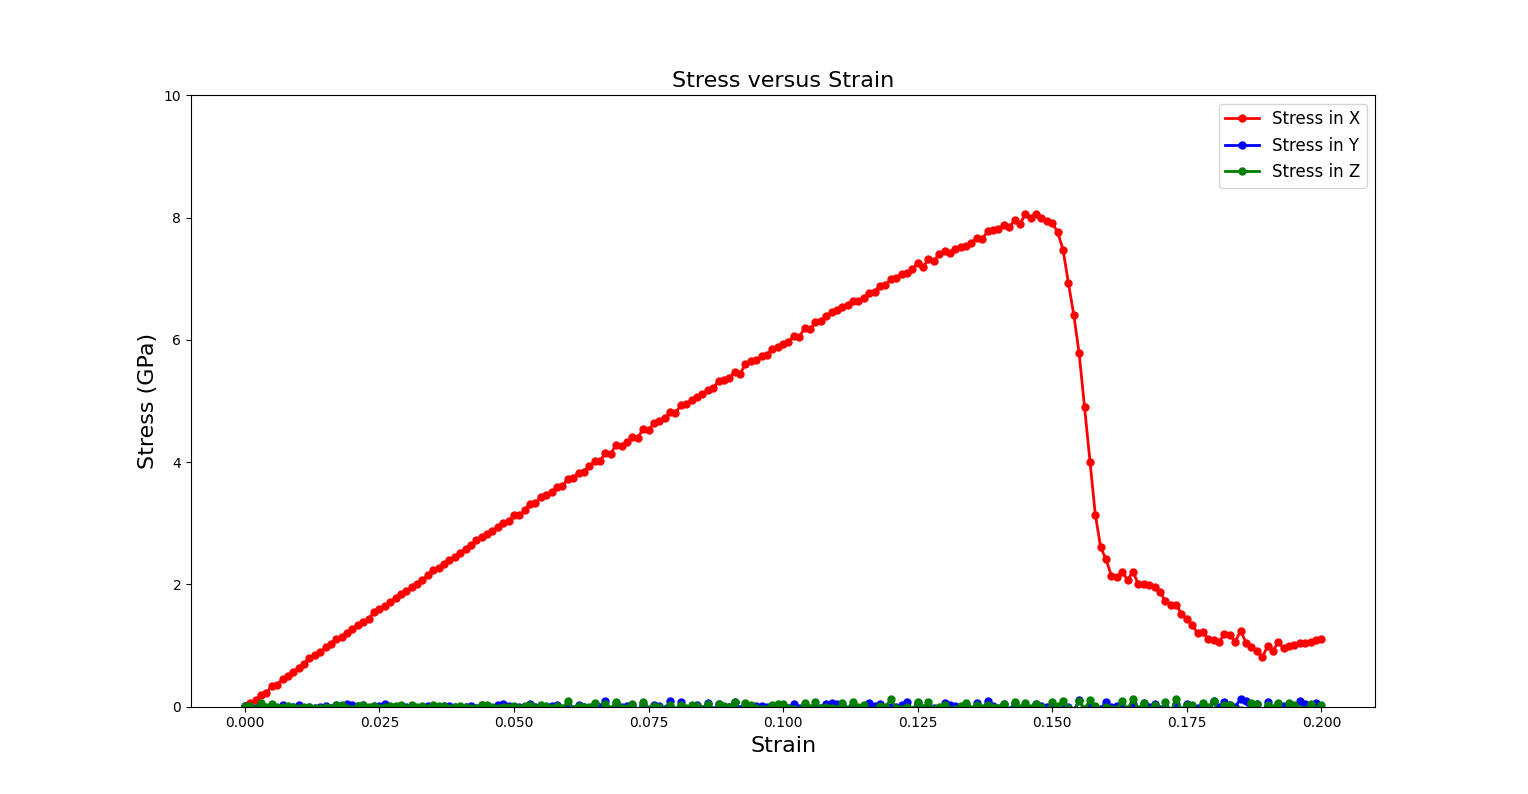
\includegraphics[height=2.20in,width=3.5in, viewport=0 0 1050 554,clip]{Lammps-Stress_Strain.png}
\caption{\fontsize{6.2pt}{5.2pt}\selectfont{\textrm{Stress-strain curve for uniaxial tensile loading of single crystal aluminum in the <100> loading direction.}}}%(与文献\cite{EPJB33-47_2003}图1对比)
\label{LAMMPS_output-Stress-Strain}
\end{figure}
}

\frame
{
	\frametitle{拉伸载荷}
\begin{figure}[h!]
\centering
\vskip -5pt
\animategraphics[autoplay, loop, height=2.40in, width=2.50in,viewport= 0 0 256 256,clip]{1}{Figures/Lammps-simulation-cell-in-tension-}{0}{81}
\caption{\fontsize{6.2pt}{5.2pt}\selectfont{\textrm{Tensile Loading of an Aluminum Single Crystal..}}}%(与文献\cite{EPJB33-47_2003}图1对比)
\label{LAMMPS_Tensile-Loading}
\end{figure}
}

\frame[allowframebreaks]
{
	\frametitle{\textrm{LAMMPS}的输入文件}
	{\fontsize{6.0pt}{5.0pt}\selectfont{
%\verbatiminput{Figures/Lammps_in_lj.txt} %为保险:~选用文件名绝对路径
\verbatiminput{Figures/Lammps_tutorial-04-Lammps-in.txt} %为保险:~选用文件名绝对路径
}}
}

\frame
{
	\frametitle{应力-应变曲线}
\begin{figure}[h!]
\centering
\vskip -5pt
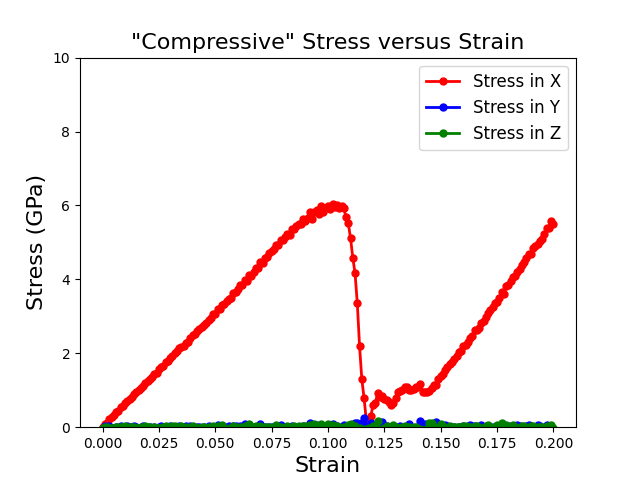
\includegraphics[height=2.40in,width=3.0in, viewport=0 0 450 354,clip]{Lammps-Compressive-Stress_Strain.png}
\caption{\fontsize{6.2pt}{5.2pt}\selectfont{\textrm{Compressive Stress-strain curve for uniaxial compression loading of single crystal aluminum in the <100> loading direction.}}}%(与文献\cite{EPJB33-47_2003}图1对比)
\label{LAMMPS_output-Stress-Strain}
\end{figure}
}

\frame
{
	\frametitle{压缩载荷}
\begin{figure}[h!]
\centering
\vskip -5pt
\animategraphics[autoplay, loop, height=2.40in, width=2.50in,viewport= 0 0 256 256,clip]{1}{Figures/Lammps-simulation-cell-in-compression-}{0}{80}
\caption{\fontsize{6.2pt}{5.2pt}\selectfont{\textrm{Compression Loading of an Aluminum Single Crystal.}}}%(与文献\cite{EPJB33-47_2003}图1对比)
\label{LAMMPS_Compression-Loading}
\end{figure}
}

\subsection{模拟晶界的形成}
\frame[allowframebreaks]
{
	\frametitle{\textrm{LAMMPS}的输入文件}
	{\fontsize{6.0pt}{5.0pt}\selectfont{
%\verbatiminput{Figures/Lammps_in_lj.txt} %为保险:~选用文件名绝对路径
\verbatiminput{Figures/Lammps_tutorial-05-Lammps-in.txt} %为保险:~选用文件名绝对路径
}}
}

\frame
{
	\frametitle{\textrm{LAMMPS}的输出文件}
\begin{figure}[h!]
\centering
\vskip -10pt
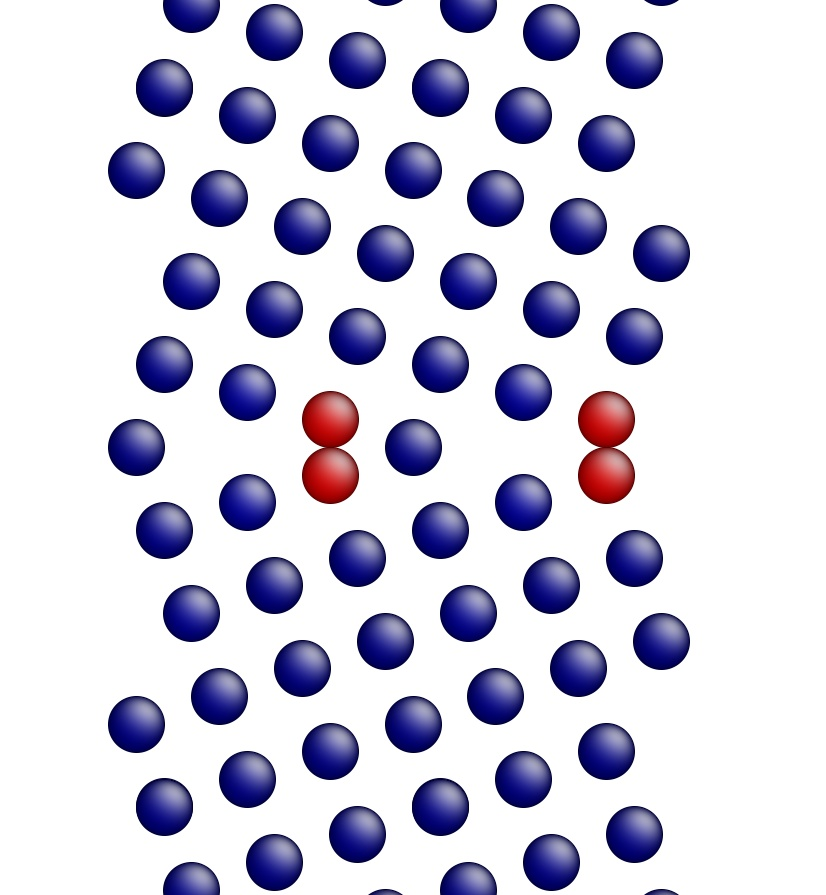
\includegraphics[height=2.40in,width=2.3in, viewport=0 0 780 890,clip]{Lammps-simulation_grain_boundary_structure-1.jpeg}
\caption{\fontsize{6.2pt}{5.2pt}\selectfont{\textrm{The grain boundary structure prior to minimization.}}}%(与文献\cite{EPJB33-47_2003}图1对比)
\label{LAMMPS_output-simulation_grain_boundary_structure-1}
\end{figure}
}

\frame
{
	\frametitle{\textrm{LAMMPS}的输出文件}
\begin{figure}[h!]
\centering
\vskip -10pt
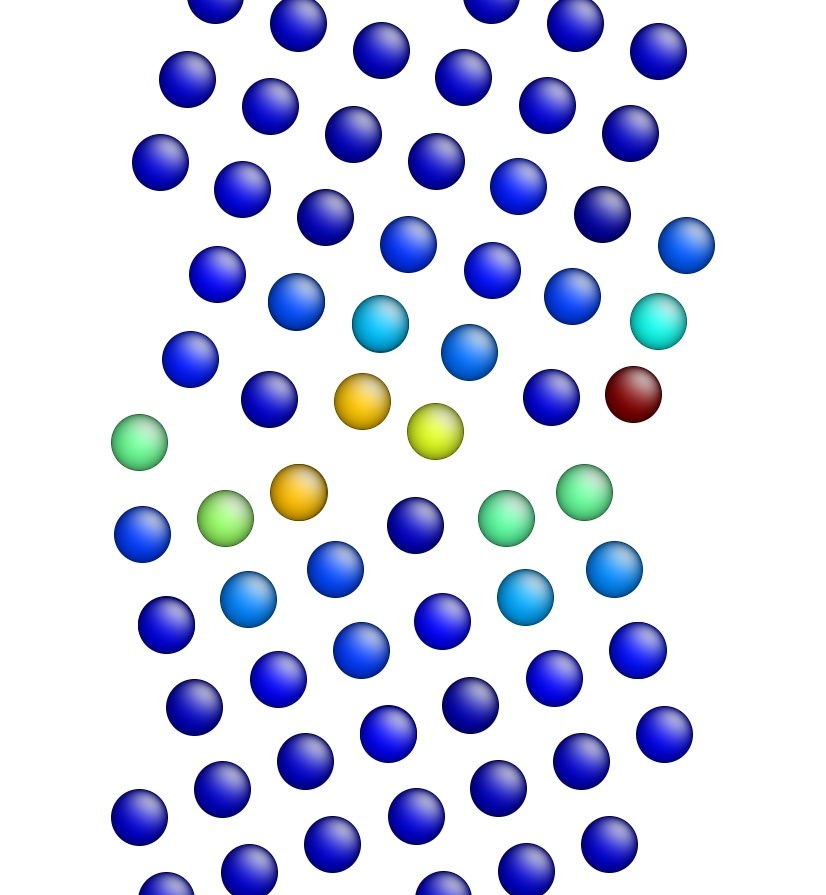
\includegraphics[height=2.40in,width=2.3in, viewport=0 0 780 890,clip]{Lammps-simulation_grain_boundary_structure-2.jpeg}
\caption{\fontsize{6.2pt}{5.2pt}\selectfont{\textrm{The grain boundary structure after minimization (overlap distance equals 0.35).}}}%(与文献\cite{EPJB33-47_2003}图1对比)
\label{LAMMPS_output-simulation_grain_boundary_structure-2}
\end{figure}
}

\frame
{
	\frametitle{\textrm{LAMMPS}的输出文件}
\begin{figure}[h!]
\centering
\vskip -10pt
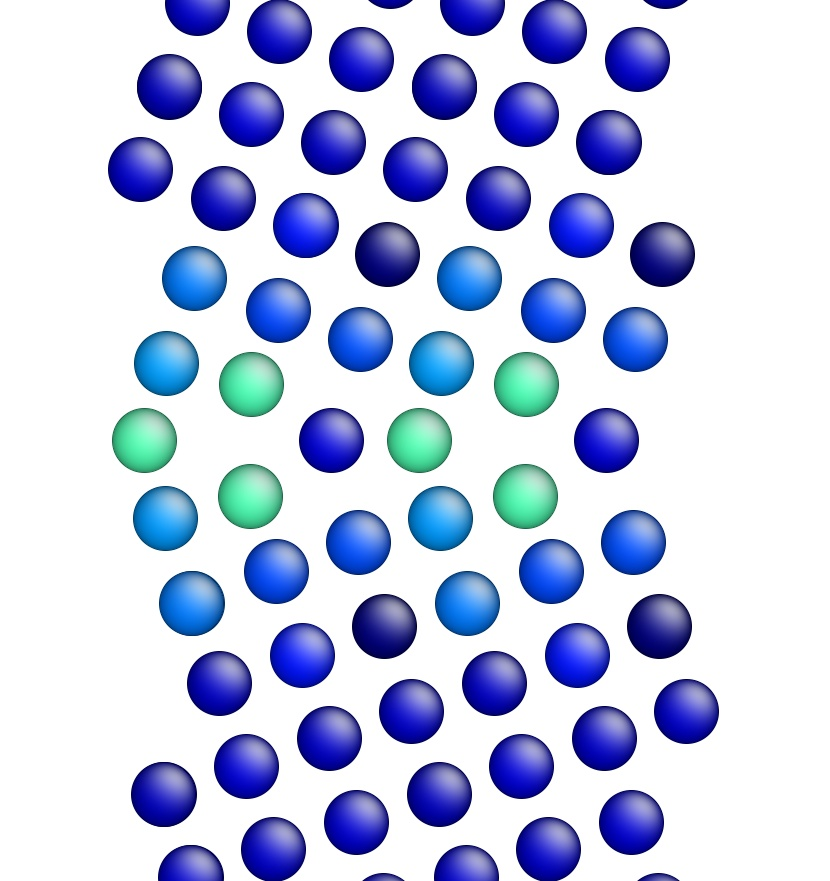
\includegraphics[height=2.40in,width=2.3in, viewport=0 0 780 890,clip]{Lammps-simulation_grain_boundary_structure-3.jpeg}
\caption{\fontsize{6.2pt}{5.2pt}\selectfont{\textrm{The grain boundary structure after minimization (overlap distance equals 1.50).}}}%(与文献\cite{EPJB33-47_2003}图1对比)
\label{LAMMPS_output-simulation_grain_boundary_structure-3}
\end{figure}
}

\frame
{
	\frametitle{\textrm{LAMMPS}的输出文件}
\begin{figure}[h!]
\centering
\vskip -10pt
\animategraphics[autoplay, loop, height=2.40in, width=2.00in,viewport= 0 0 400 470,clip]{1}{Figures/Lammps-simulation_grain_boundary-for-aluminum-1-}{0}{31}
\caption{\fontsize{6.2pt}{5.2pt}\selectfont{\textrm{The minimization of the grain boundary structure for an aluminum $\Sigma5(310)$ symmetric tilt grain boundary.}}}%(与文献\cite{EPJB33-47_2003}图1对比)
\label{LAMMPS_output-simulation_fracture-of-Fe}
\end{figure}
}

\frame
{
	\frametitle{\textrm{LAMMPS}的输出文件}
\begin{figure}[h!]
\centering
\vskip -10pt
\animategraphics[autoplay, loop, height=2.40in, width=2.00in,viewport= 0 0 400 470,clip]{1}{Figures/Lammps-simulation_grain_boundary-for-aluminum-2-}{0}{16}
\caption{\fontsize{6.2pt}{5.2pt}\selectfont{\textrm{The minimization of the grain boundary structure for an aluminum $\Sigma5(310)$ symmetric tilt grain boundary (with a slightly different starting position.).}}}%(与文献\cite{EPJB33-47_2003}图1对比)
\label{LAMMPS_output-simulation_fracture-of-Fe}
\end{figure}
}

\subsection{拉伸晶界直至断裂}
\frame[allowframebreaks]
{
	\frametitle{\textrm{LAMMPS}的输入文件}
	{\fontsize{6.0pt}{5.0pt}\selectfont{
%\verbatiminput{Figures/Lammps_in_lj.txt} %为保险:~选用文件名绝对路径
\verbatiminput{Figures/Lammps_tutorial-06-Lammps-in.txt} %为保险:~选用文件名绝对路径
}}
}

\frame
{
	\frametitle{\textrm{LAMMPS}的输出文件}
\begin{figure}[h!]
\centering
\vskip -10pt
\animategraphics[autoplay, loop, height=2.40in, width=1.10in,viewport= 30 0 170 260,clip]{1}{Figures/Lammps-simulation_fracture-of-Fe-}{0}{120}
\caption{\fontsize{6.2pt}{5.2pt}\selectfont{\textrm{The fracture of a Fe symmetric tilt grain boundary. Atoms are colored by the stress in the y-direction.}}}%(与文献\cite{EPJB33-47_2003}图1对比)
\label{LAMMPS_output-simulation_fracture-of-Fe}
\end{figure}
}

\subsection{铁的对称倾转晶界断裂的原子模拟}
\frame[allowframebreaks]
{
	\frametitle{\textrm{LAMMPS}的输入文件}
	{\fontsize{6.0pt}{5.0pt}\selectfont{
%\verbatiminput{Figures/Lammps_in_lj.txt} %为保险:~选用文件名绝对路径
\verbatiminput{Figures/Lammps_tutorial-07-Lammps-in.txt} %为保险:~选用文件名绝对路径
}}
}

\frame[allowframebreaks]
{
	\frametitle{\textrm{LAMMPS}的\textrm{data}文件}
	{\fontsize{6.0pt}{5.0pt}\selectfont{
%\verbatiminput{Figures/Lammps_in_lj.txt} %为保险:~选用文件名绝对路径
\verbatiminput{Figures/Lammps_tutorial-07-Lammps-data.txt} %为保险:~选用文件名绝对路径
}}
}

\frame
{
	\frametitle{\textrm{LAMMPS}的输出文件}
\begin{figure}[h!]
\centering
\vskip -5pt
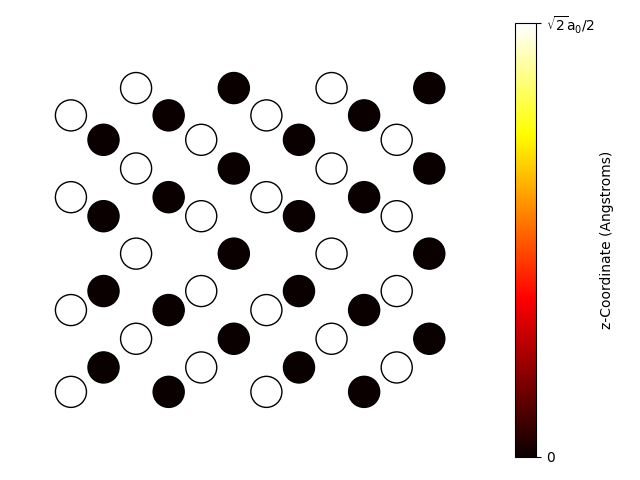
\includegraphics[height=2.40in,width=3.4in, viewport=0 0 450 354,clip]{Lammps-grain_boundary-for-atoms-1.png}
\caption{\fontsize{6.2pt}{5.2pt}\selectfont{\textrm{The atoms colored by the in-plane coordinate (z-direction:~the black and white grain boundary structure look for atoms that sit on different \{110\} planes).}}}%(与文献\cite{EPJB33-47_2003}图1对比)
\label{LAMMPS_output-grain_boundary-for-atoms-1}
\end{figure}
}

%\frame
%{
%	\frametitle{\textrm{LAMMPS}的输出文件}
%\begin{figure}[h!]
%\centering
%\vskip -5pt
%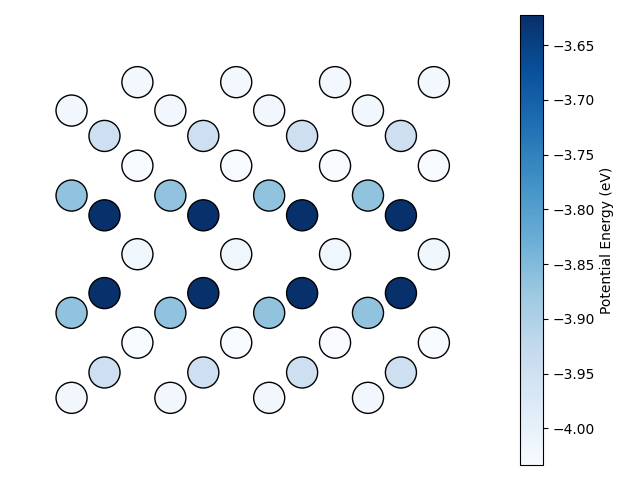
\includegraphics[height=2.40in,width=3.0in, viewport=0 0 450 354,clip]{Lammps-grain_boundary-for-atoms-2.png}
%\caption{\fontsize{6.2pt}{5.2pt}\selectfont{\textrm{The atoms colored by the in-plane coordinate (z-direction:~the black and white grain boundary structure look for atoms that sit on different \{110\} planes).}}}%(与文献\cite{EPJB33-47_2003}图1对比)
%\label{LAMMPS_output-grain_boundary-for-atoms-2}
%\end{figure}
%}
%
\subsection{长链聚合物行为模拟}
\frame[allowframebreaks]
{
	\frametitle{\textrm{LAMMPS}的\textrm{data}文件}
	{\fontsize{6.0pt}{5.0pt}\selectfont{
%\verbatiminput{Figures/Lammps_in_lj.txt} %为保险:~选用文件名绝对路径
\verbatiminput{Figures/Lammps_tutorial-08-Lammps-data.txt} %为保险:~选用文件名绝对路径
}}
}

\frame
{
	\frametitle{\textrm{LAMMPS}中的键角与二面角}
\begin{figure}[h!]
\centering
\vskip -5pt
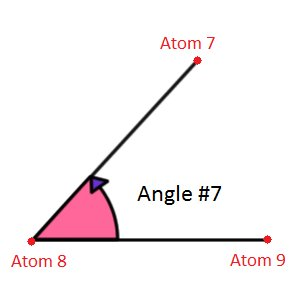
\includegraphics[height=1.70in,width=1.9in, viewport=0 0 320 280,clip]{Lammps-Angles_between_atoms.jpeg}
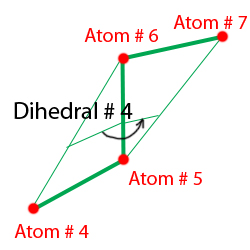
\includegraphics[height=1.70in,width=1.9in, viewport=0 0 280 250,clip]{Lammps-Dihedral_angles_between_atoms.jpeg}
\caption{\fontsize{6.2pt}{5.2pt}\selectfont{\textrm{A schematic of angles~(left) and dihedral angles~(right) between atoms defined in LAMMPS.}}}%(与文献\cite{EPJB33-47_2003}图1对比)
\label{LAMMPS_Angle-and-Dihedral_angle}
\end{figure}
}

\frame[allowframebreaks]
{
	\frametitle{\textrm{LAMMPS}的输入文件}
	{\fontsize{6.0pt}{5.0pt}\selectfont{
%\verbatiminput{Figures/Lammps_in_lj.txt} %为保险:~选用文件名绝对路径
\verbatiminput{Figures/Lammps_tutorial-08-Lammps-in.txt} %为保险:~选用文件名绝对路径
}}
}

\frame
{
	\frametitle{\textrm{LAMMPS}的输出文件}
\begin{figure}[h!]
\centering
\vskip -5pt
\animategraphics[autoplay, loop, height=2.40in, width=2.50in,viewport= 0 0 556 536,clip]{1}{Figures/Lammps-simulation_Equilibration-process-followed-by-minimization-}{0}{211}
\caption{\fontsize{6.2pt}{5.2pt}\selectfont{\textrm{Equilibration process followed by minimization for a single polymer chain.}}}%(与文献\cite{EPJB33-47_2003}图1对比)
\label{LAMMPS_output-Equilibration-process-followed-by-minimization}
\end{figure}
}
%\vskip 5pt
\section{模型算例}
\subsection{金纳米线的断裂模拟}
\frame[allowframebreaks]
{
	\frametitle{\textrm{LAMMPS}的输入文件}
	{\fontsize{6.0pt}{5.0pt}\selectfont{
\verbatiminput{Figures/Lammps_tutorial-11-in.txt} %为保险:~选用文件名绝对路径
}}
}

\frame
{
	\frametitle{金纳米线的断裂模拟}
\begin{figure}[h!]
\centering
\vskip -5pt
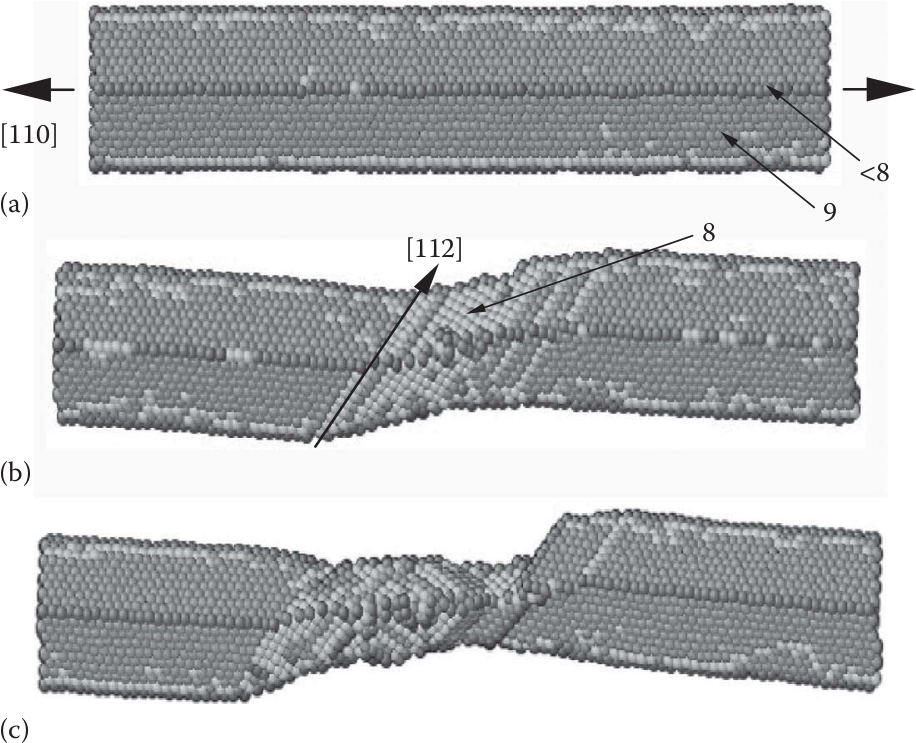
\includegraphics[height=2.40in,width=4.0in, viewport=0 0 940 740,clip]{Lammps_tutorial-11-tensile_loading.png}
\caption{\fontsize{6.2pt}{5.2pt}\selectfont{\textrm{Deformation behavior of an Au nanowire during tensile loading. Timestep=0~(a), 150,000~(b), 282,000~(c).}}}%(与文献\cite{EPJB33-47_2003}图1对比)
\label{LAMMPS_Au-nanowire}
\end{figure}
}

\subsection{纳米水粒滴被石墨烯纳米带的自发包裹}
\frame[allowframebreaks]
{
	\frametitle{\textrm{LAMMPS}的输入文件}
	{\fontsize{6.0pt}{5.0pt}\selectfont{
\verbatiminput{Figures/Lammps_tutorial-12-in.txt} %为保险:~选用文件名绝对路径
}}
}

\frame[allowframebreaks]
{
	\frametitle{\textrm{LAMMPS}的\textrm{data}文件}
	{\fontsize{6.0pt}{5.0pt}\selectfont{
%\verbatiminput{Figures/Lammps_in_lj.txt} %为保险:~选用文件名绝对路径
\verbatiminput{Figures/Lammps_tutorial-12-data.txt} %为保险:~选用文件名绝对路径
}}
}

\frame
{
	\frametitle{纳米水粒滴的自发包裹}
\begin{figure}[h!]
\centering
\vskip -5pt
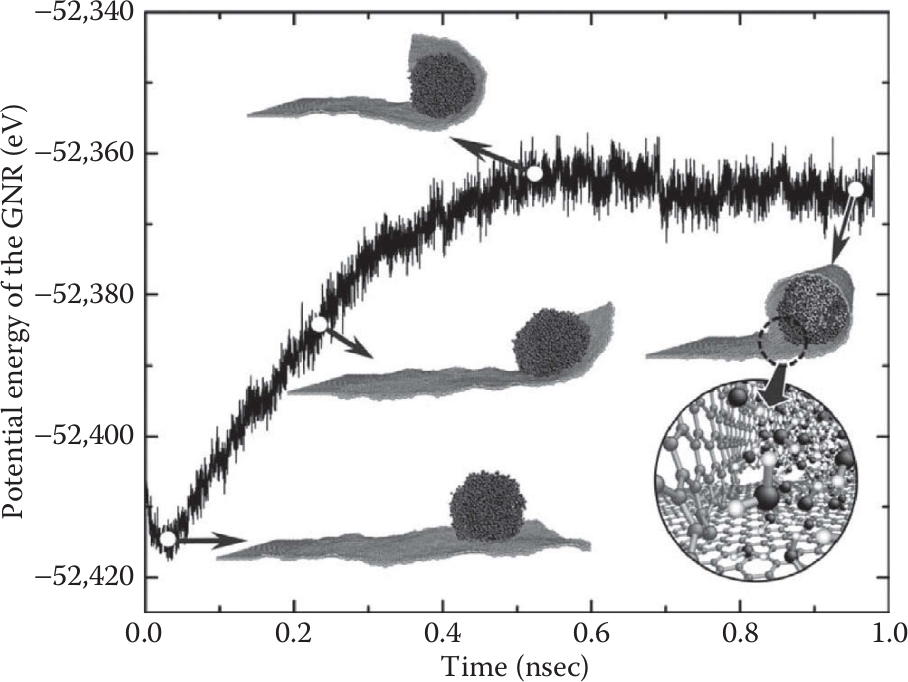
\includegraphics[height=2.40in,width=3.1in, viewport=0 0 940 700,clip]{Lammps_tutorial-12-spontaneous_wrapping.png}
\caption{\fontsize{6.2pt}{5.2pt}\selectfont{\textrm{Spontaneous wrapping of a water nanodroplet by the GNR.}}}%(与文献\cite{EPJB33-47_2003}图1对比)
\label{LAMMPS_water-nanodroplet-spontaneous-wrapping-GNR}
\end{figure}
}

\subsection{碳纳米管的拉伸}
\frame[allowframebreaks]
{
	\frametitle{\textrm{LAMMPS}的输入文件}
	{\fontsize{6.0pt}{5.0pt}\selectfont{
\verbatiminput{Figures/Lammps_tutorial-13-in.txt} %为保险:~选用文件名绝对路径
}}
}

\frame[allowframebreaks]
{
	\frametitle{\textrm{LAMMPS}的\textrm{data}文件}
	{\fontsize{6.0pt}{5.0pt}\selectfont{
%\verbatiminput{Figures/Lammps_in_lj.txt} %为保险:~选用文件名绝对路径
\verbatiminput{Figures/Lammps_tutorial-13-data.txt} %为保险:~选用文件名绝对路径
}}
}

\frame
{
	\frametitle{碳纳米管的断裂模拟}
\begin{figure}[h!]
\centering
\vskip -5pt
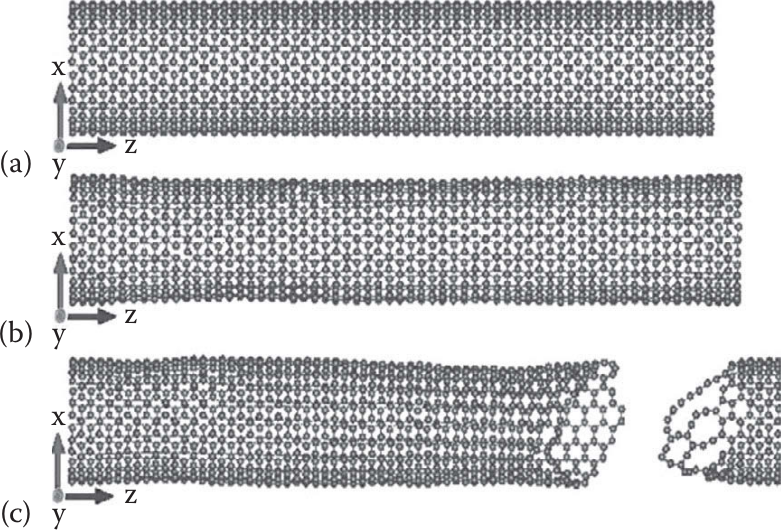
\includegraphics[height=2.40in,width=3.5in, viewport=0 0 820 520,clip]{Lammps_tutorial-13-Fracture_of_a_CNT_under_tension.png}
\caption{\fontsize{6.2pt}{5.2pt}\selectfont{\textrm{Fracture of a CNT under tension at timesteps of 0~(a), 20,000~(b), 40,000~(c).}}}%(与文献\cite{EPJB33-47_2003}图1对比)
\label{LAMMPS_Frcture-of-CNT-under_ternsion}
\end{figure}
}

\frame
{
	\frametitle{拉伸条件下碳纳米管的应力-应变}
\begin{figure}[h!]
\centering
\vskip -5pt
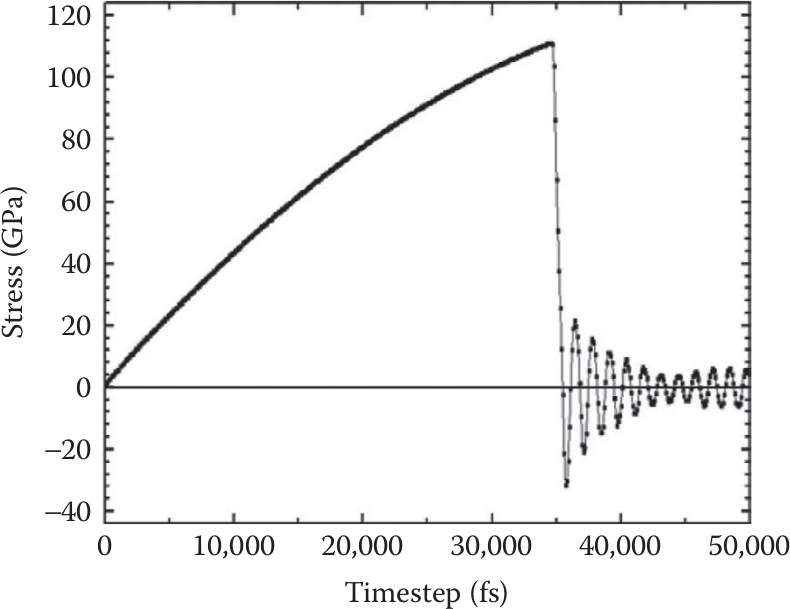
\includegraphics[height=2.40in,width=3.1in, viewport=0 0 820 620,clip]{Lammps_tutorial-13-Stress_strain-curve-of-a-CNT_under_tension.png}
\caption{\fontsize{6.2pt}{5.2pt}\selectfont{\textrm{Stress–strain curve of a CNT under tension.}}}%(与文献\cite{EPJB33-47_2003}图1对比)
\label{LAMMPS_Stress_strain-of-CNT_under_tension}
\end{figure}
}

\subsection{硅柱的拉伸裂纹}
\frame[allowframebreaks]
{
	\frametitle{\textrm{LAMMPS}的输入文件}
	{\fontsize{6.0pt}{5.0pt}\selectfont{
\verbatiminput{Figures/Lammps_tutorial-14-in.txt} %为保险:~选用文件名绝对路径
}}
}

\frame
{
	\frametitle{硅柱的断纹模拟}
\begin{figure}[h!]
\centering
\vskip -15pt
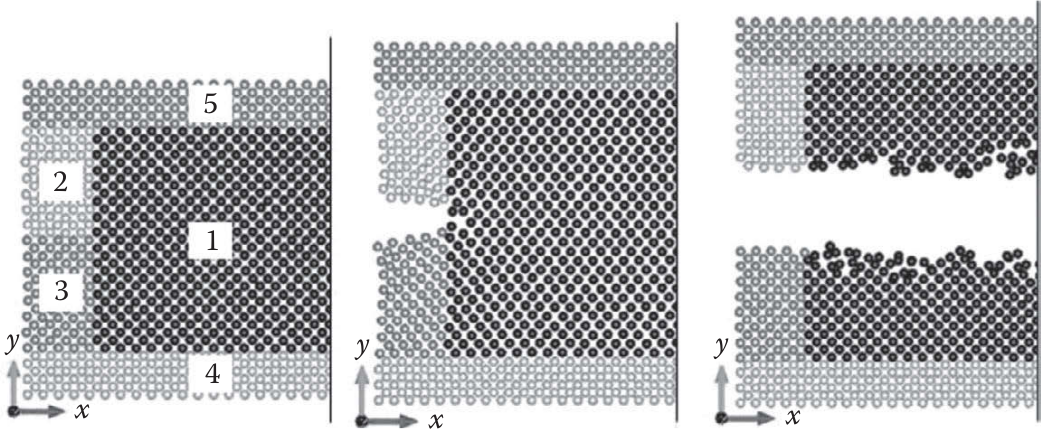
\includegraphics[height=2.10in,width=4.0in, viewport=0 0 1050 500,clip]{Lammps_tutorial-14-Si_crack-initiating-block_under_tension.png}
\caption{\fontsize{6.2pt}{5.2pt}\selectfont{\textrm{Si bar with a small crack-initiating block under tension: at timesteps of 0~(a), 15,000~(b), 25,000~(c).}}}%(与文献\cite{EPJB33-47_2003}图1对比)
\label{LAMMPS_Si_bar-Crack-initiating_block_under_tension}
\end{figure}
}

\frame
{
	\frametitle{拉伸裂纹与硅柱的应力-应变}
\begin{figure}[h!]
\centering
\vskip -5pt
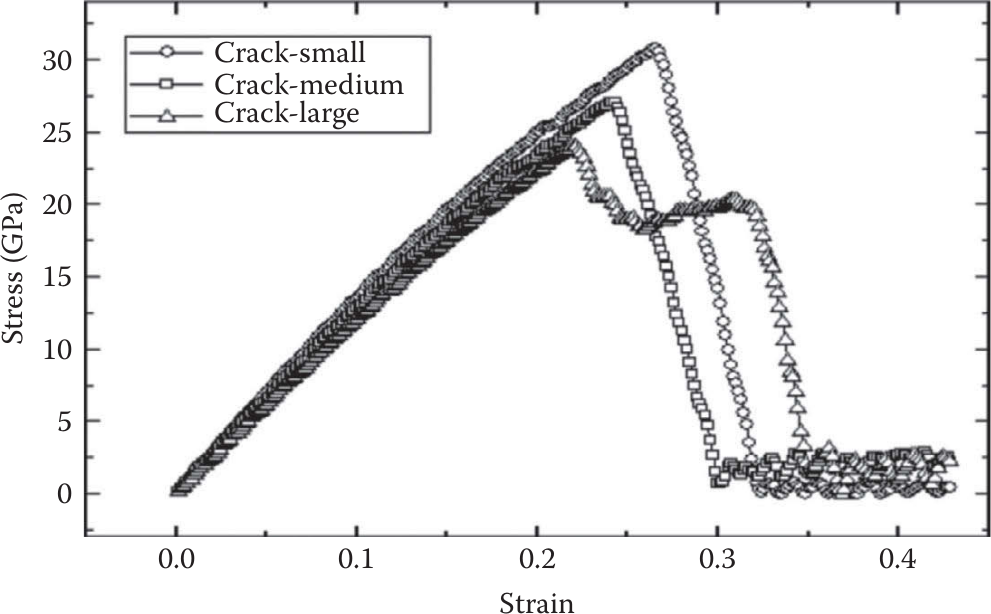
\includegraphics[height=2.40in,width=3.5in, viewport=0 0 1000 620,clip]{Lammps_tutorial-14-Stress_strain-curves-Si_crack-initiating-block_under_tension.png}
\caption{\fontsize{6.2pt}{5.2pt}\selectfont{\textrm{Stress–strain curve of Si bars with various initial crack sizes.}}}%(与文献\cite{EPJB33-47_2003}图1对比)
\label{LAMMPS_Stress_strain-of-Si_bar-with-various_initial_crack_sizes}
\end{figure}
}

\subsection{硅-碳纳米管复合材料的拉伸}
\frame
{
	\frametitle{硅-碳纳米管复合材料的设计}
\begin{figure}[h!]
\centering
\vskip -8pt
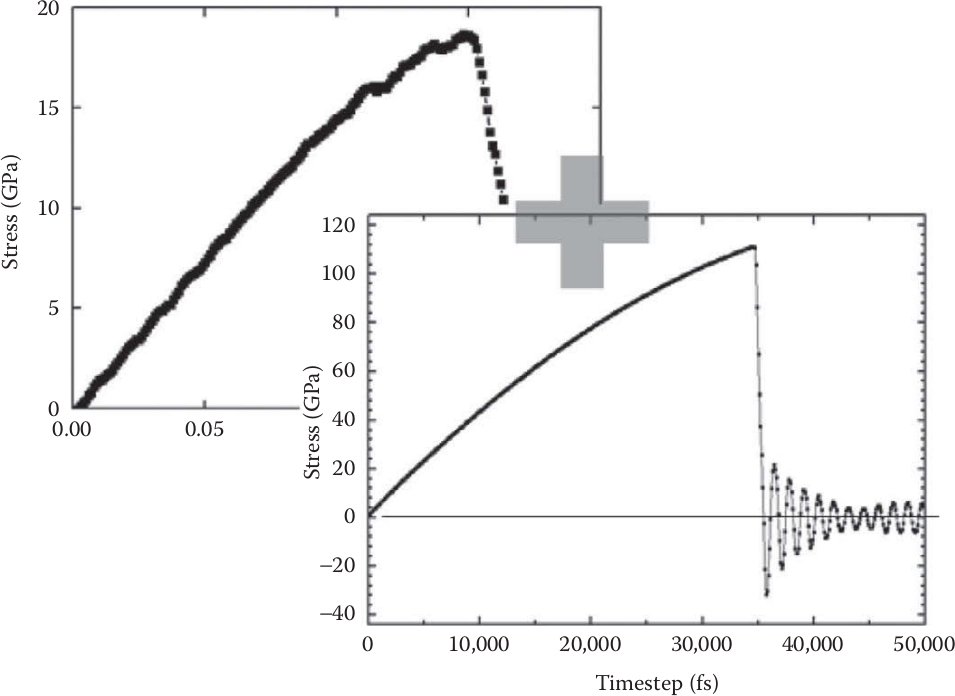
\includegraphics[height=2.70in,width=3.6in, viewport=0 0 960 700,clip]{Lammps_tutorial-15-design_concept-for-the-Si-CNT.png}
\caption{\fontsize{6.2pt}{5.2pt}\selectfont{\textrm{Design concept for the Si–CNT composite system.}}}%(与文献\cite{EPJB33-47_2003}图1对比)
\label{LAMMPS_Design_concept-for-Si_CNT.}
\end{figure}
}

\frame[allowframebreaks]
{
	\frametitle{\textrm{LAMMPS}的输入文件}
	{\fontsize{6.0pt}{5.0pt}\selectfont{
\verbatiminput{Figures/Lammps_tutorial-15-in.txt} %为保险:~选用文件名绝对路径
}}
}

\frame
{
	\frametitle{硅-碳纳米管复合材料的初始结构}
\begin{figure}[h!]
\centering
\vskip -10pt
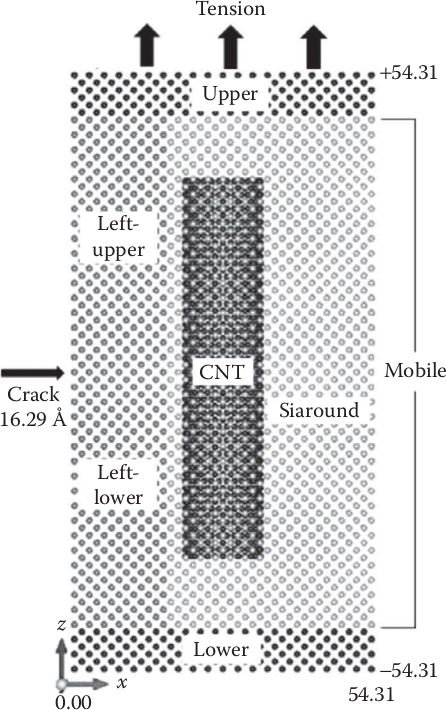
\includegraphics[height=2.70in,width=2.1in, viewport=0 0 500 720,clip]{Lammps_tutorial-15-starting_structure-for-the-Si-CNT.png}
\caption{\fontsize{6.2pt}{5.2pt}\selectfont{\textrm{Starting structure of the Si–CNT composite system.}}}%(与文献\cite{EPJB33-47_2003}图1对比)
\label{LAMMPS_Starting-structure-of-Si_CNT.}
\end{figure}
}

\frame[allowframebreaks]
{
	\frametitle{\textrm{LAMMPS}的\textrm{data}文件}
	{\fontsize{6.0pt}{5.0pt}\selectfont{
%\verbatiminput{Figures/Lammps_in_lj.txt} %为保险:~选用文件名绝对路径
\verbatiminput{Figures/Lammps_tutorial-15-data.txt} %为保险:~选用文件名绝对路径
}}
}

\frame
{
	\frametitle{硅-碳纳米管复合材料的原子间相互作用}
\begin{figure}[h!]
\centering
\vskip -5pt
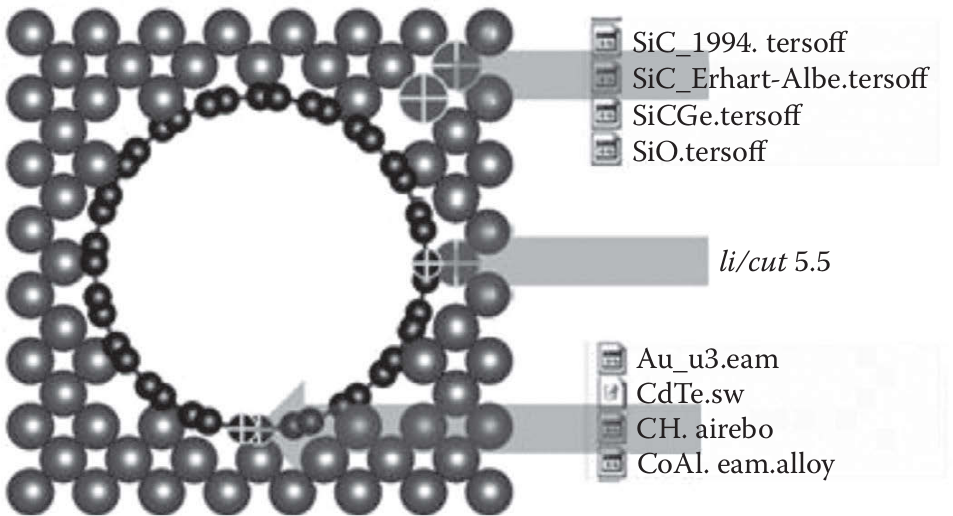
\includegraphics[height=2.40in,width=4.0in, viewport=0 0 940 540,clip]{Lammps_tutorial-15-three_potentials-adopted-for_Si-CNT_and_their-interface.png}
\caption{\fontsize{6.2pt}{5.2pt}\selectfont{\textrm{Three potentials adopted for the study to describe Si, CNT, and their interface.}}}%(与文献\cite{EPJB33-47_2003}图1对比)
\label{LAMMPS_Potential-Si-CNT}
\end{figure}
}

\frame
{
	\frametitle{硅-碳纳米管复合材料的拉伸过程}
\begin{figure}[h!]
\centering
\vskip -10pt
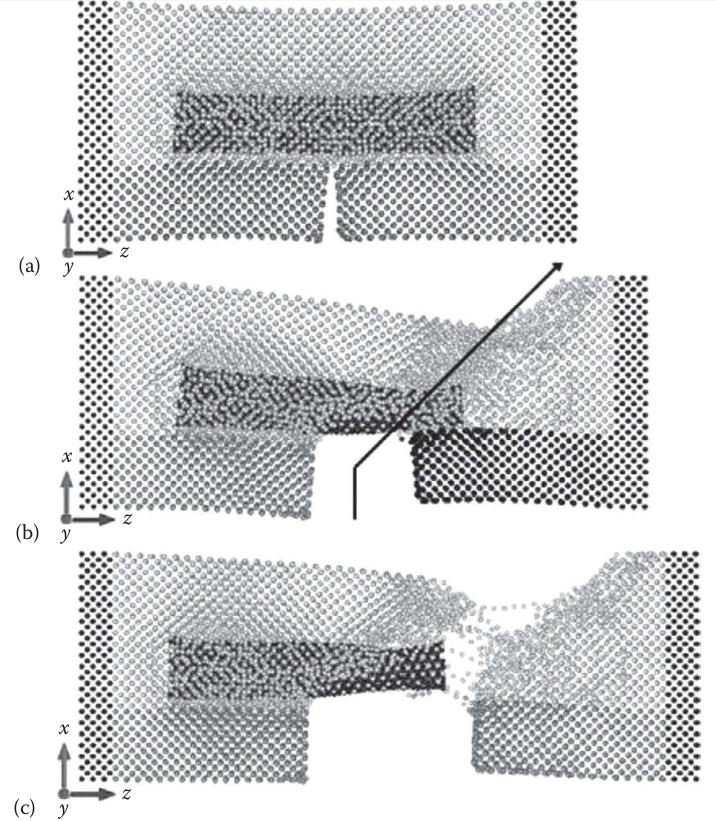
\includegraphics[height=2.60in,width=2.8in, viewport=0 0 770 820,clip]{Lammps_tutorial-15-snapshots_of_the Si-CNT_composite_system_under-tension-for-various-strains.png}
\caption{\fontsize{6.2pt}{5.2pt}\selectfont{\textrm{Snapshots of the Si–CNT composite system with $\varepsilon=0.5\mathrm{eV}$ under tension for various strains:~10.5\%~(a), 31.5\%~(b), 42\%~(c).}}}%(与文献\cite{EPJB33-47_2003}图1对比)
\label{LAMMPS_Si_CNT-under-tension}
\end{figure}
}

\frame
{
	\frametitle{硅-碳纳米管复合材料拉伸的应力-应变}
\begin{figure}[h!]
\centering
\vskip -5pt
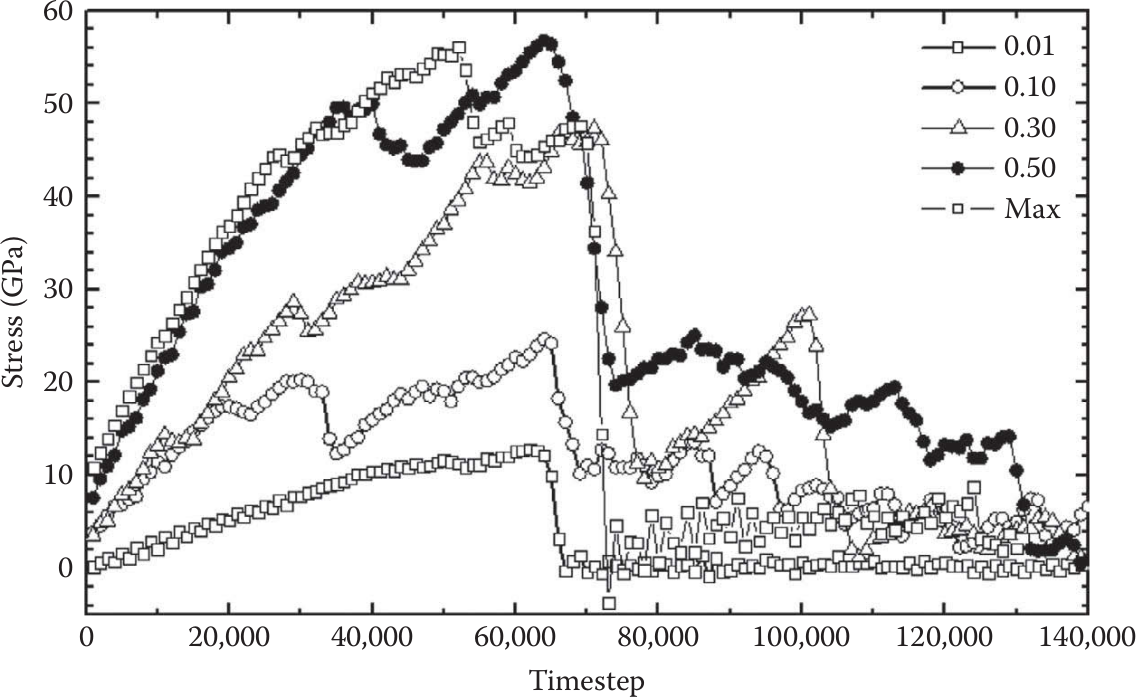
\includegraphics[height=2.42in,width=4.0in, viewport=0 0 1200 730,clip]{Lammps_tutorial-15-Stress_strain-curves-of-the-Si-CNT.png}
\caption{\fontsize{6.2pt}{5.2pt}\selectfont{\textrm{Stress–strain curves of the Si–CNT nanocomposites with various interfacial bonding strengths.}}}%(与文献\cite{EPJB33-47_2003}图1对比)
\label{LAMMPS_Stress-train-curve}
\end{figure}
}

\subsection{$\mathrm{ZrO}_2$-\rm{8}-$\mathrm{Y}_2\mathrm{O}_3$的均方位移}
\frame[allowframebreaks]
{
	\frametitle{\textrm{LAMMPS}的输入文件}
	{\fontsize{6.0pt}{5.0pt}\selectfont{
\verbatiminput{Figures/Lammps_tutorial-16-in.txt} %为保险:~选用文件名绝对路径
}}
}

\frame
{
	\frametitle{$\mathrm{ZrO}_2$-\textrm{8}$\mathrm{Y}_2\mathrm{O}_3$的结构}
\begin{figure}[h!]
\centering
\vskip -5pt
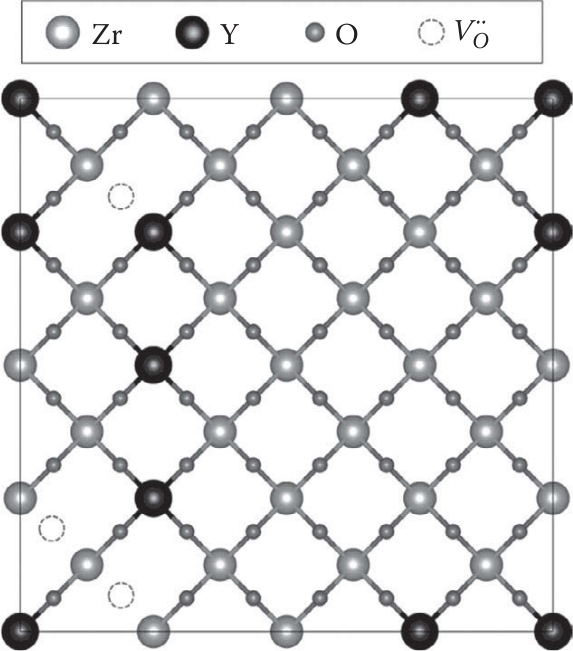
\includegraphics[height=2.40in,width=2.3in, viewport=0 0 640 680,clip]{Lammps_tutorial-16-sliced-structure-of-ZrO2-8Y2O3-system.png}
\caption{\fontsize{6.2pt}{5.2pt}\selectfont{\textrm{Sliced structure of the $\mathrm{ZrO}_2$-8$\mathrm{Y_2O_3}$ system showing a metal ($\mathrm{Zr}$ and $\mathrm{Y}$) layer and an oxygen layer along the [001] direction.}}}%(与文献\cite{EPJB33-47_2003}图1对比)
\label{LAMMPS_slice-structure-of-ZrO2-8Y2O3}
\end{figure}
}

\frame[allowframebreaks]
{
	\frametitle{\textrm{LAMMPS}的\textrm{data}文件}
	{\fontsize{6.0pt}{5.0pt}\selectfont{
%\verbatiminput{Figures/Lammps_in_lj.txt} %为保险:~选用文件名绝对路径
\verbatiminput{Figures/Lammps_tutorial-16-data.txt} %为保险:~选用文件名绝对路径
}}
}

\frame
{
	\frametitle{均方位移\textrm{(Mean-Squared Displacement,MSD)}}
\begin{figure}[h!]
\centering
\vskip -5pt
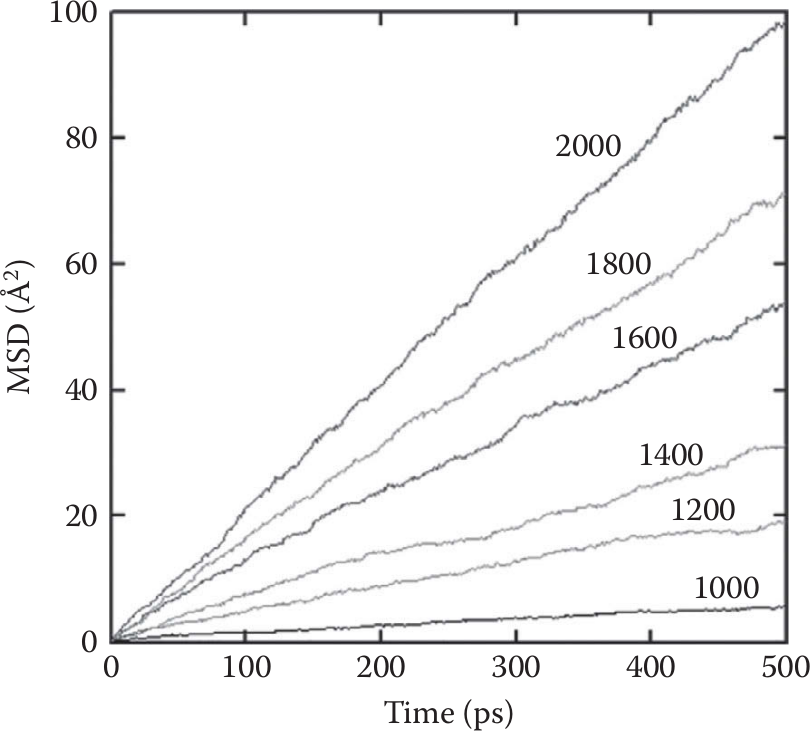
\includegraphics[height=2.50in,width=3.2in, viewport=0 0 850 780,clip]{Lammps_tutorial-16-MSD_plot-with-time_in-the_last_500000-timesteps.png}
\caption{\fontsize{6.2pt}{5.2pt}\selectfont{\textrm{MSD plot with time in the range of the last 500,000 timesteps at various temperatures from 2,000 to 1,000 K.}}}%(与文献\cite{EPJB33-47_2003}图1对比)
\label{LAMMPS_MSD-ZrO2-8Y2O3.}
\end{figure}
}

\section{\rm{LAMMPS}常用命令}
\frame
{
	\frametitle{\textcolor{cyan}{\textit{units}}:~定义单位类型}
	\begin{itemize}
		\item \textcolor{cyan}{\textit{units}}~命令用来定义模拟过程中使用的单位类型\\
			{\fontsize{7.5pt}{5.2pt}\selectfont{它决定了所有输入脚本、数据文件和所有输出到屏幕、日志文件以及\textrm{dump}文件中物理量的单位}}
		\item 语法:~\textcolor{cyan}{\textit{units}} \textrm{style}
\vskip 3pt
\textrm{styly}可取\textrm{\textcolor{magenta}{lj} or \textcolor{magenta}{real} or \textcolor{magenta}{metal} or \textcolor{magenta}{si} or \textcolor{magenta}{cgs} or \textcolor{magenta}{electron} or \textcolor{magenta}{micro} or \textcolor{magenta}{nano}}\\
{\fontsize{7.5pt}{5.2pt}\selectfont{金属中一般用\textrm{metal}}}
	\end{itemize}
}

\frame
{
	\frametitle{\textcolor{cyan}{\textit{boundary}}:~设置模拟\textrm{box}的边界条件}
	\begin{itemize}
		\item 语法:~\textcolor{cyan}{\textit{boundary}} \textrm{$x$~$y$~$z$}
\vskip 3pt
\textcolor{cyan}{\textit{boundary}}命令设置box的边界条件,参数\textrm{$x$~$y$~$z$}分别设置该维度的边界条件,最基本的边界条件有四种:~\textrm{\textcolor{blue}{p}~\textcolor{blue}{f}~\textcolor{blue}{s}~\textcolor{blue}{m}}
	\begin{itemize}

{\fontsize{7.5pt}{5.2pt}\selectfont{
		\item \textrm{\textcolor{blue}{p}}是周期性边界:~当粒子从一侧飞出,会从相对应的另一侧再次进入\textrm{box},一般情况下不会发生\textrm{''lost~atoms''}(丢失原子)错误
		\item \textrm{\textcolor{blue}{f}}是固定边界:~表示\textrm{box}的表面在该方向上被固定住,不因体系压力的变化发生移动,如果原子从一个表面飞出,会提示\textrm{''lost~atoms''}错误\\
			{\fontsize{6.2pt}{5.2pt}\selectfont{设置\textcolor{cyan}{\textit{thermo\_modify}}~\textrm{\textcolor{blue}{lost}}可以允许原子丢失,否则模拟过程会被终止}}
		\item \textrm{\textcolor{blue}{s}}是收缩性边界条件:~表示在该方向上,盒子的表面会根据体系的压力大小或原子运动情况发生移动\\
			{\fontsize{6.2pt}{5.2pt}\selectfont{一般情况下,盒子会配合原子的移动,尽量把原子包含在\textrm{box}内,但是当原子速度过快,位移太大时原子也可能会飞出盒子,造成\textrm{''lost~atoms''}错误}}}}
	\end{itemize}
{\fontsize{7.0pt}{5.2pt}\selectfont{
	\textrm{LAMMPS}支持对同一方向的两个边界设置不同的边界条件,对$y$方向下表面设置\textrm{\textcolor{blue}{f}}边界、上表面设置\textrm{\textcolor{blue}{s}}边界,可以写为:\\
	\textcolor{cyan}{\textit{boundary}}~ \textcolor{blue}{\textrm{p}}~\textcolor{blue}{\textrm{fs}}~\textcolor{blue}{\textrm{p}}}}
	\end{itemize}
}

\frame
{
	\frametitle{\textcolor{cyan}{\textit{atom\_style}}:~定义模拟过程中原子的类型}
	\begin{itemize}
		\item 语法:~\textcolor{cyan}{\textit{atom\_style}} \textrm{\textcolor{blue}{style}}\\
			\textrm{\textcolor{blue}{style}}为\textrm{\textcolor{magenta}{amoeba} or \textcolor{magenta}{angle} or \textcolor{magenta}{atomic} or \textcolor{magenta}{body} or \textcolor{magenta}{bond} or \textcolor{magenta}{charge} or \textcolor{magenta}{dipole} or \textcolor{magenta}{dpd} or \textcolor{magenta}{edpd} or \textcolor{magenta}{electron} or \textcolor{magenta}{ellipsoid} or \textcolor{magenta}{full} or \textcolor{magenta}{line} or \textcolor{magenta}{mdpd} or \textcolor{magenta}{molecular} or \textcolor{magenta}{oxdna} or \textcolor{magenta}{peri} or \textcolor{magenta}{smd} or \textcolor{magenta}{sph} or \textcolor{magenta}{sphere} or \textcolor{magenta}{bpm}/\textcolor{magenta}{sphere} or \textcolor{magenta}{spin} or \textcolor{magenta}{tdpd} or \textcolor{magenta}{tri} or \textcolor{magenta}{template} or \textcolor{magenta}{hybrid}}
		\item \textcolor{cyan}{atom\_style}命令用来定义模拟过程中原子的类型:~不同的对象粒子所具有的属性不同
	\end{itemize}
{\fontsize{7.5pt}{5.2pt}\selectfont{
	\textcolor{red}{对于某个粒子对象,粒子不存在的属性就不需要设置,以便节省内存,加速运算}}}
\vskip 5pt
{\fontsize{6.2pt}{5.2pt}\selectfont{
当\textrm{style}为\textcolor{blue}{\textrm{full}}时,其属性包括:~粒子编号,粒子所属分子的编号,粒子类别\textrm{(atom type)},带电电荷量,坐标$x$,$y$,$z$\\
如果粒子是金属粒子,如\textrm{Fe},粒子\textrm{style}为\textcolor{blue}{\textrm{atomic}}的属性是:~粒子编号,粒子类别,坐标$x$,$y$,$z$}}
}

\frame
{
	\frametitle{\textcolor{cyan}{\textit{variable}}:~定义一个变量}
	\begin{itemize}
		\item 语法:~\textcolor{cyan}{\textit{variable}} \textrm{\textcolor{blue}{name style $\cdots$}}\\
			{\fontsize{7.5pt}{5.2pt}\selectfont{\textcolor{blue}{\textrm{name}}是用户定义的变量名}}\\
			\textrm{\textcolor{blue}{style}}是变量类型,可以为\textrm{\textcolor{magenta}{delete} or \textcolor{magenta}{index} or \textcolor{magenta}{loop} or \textcolor{magenta}{world} or \textcolor{magenta}{universe} or \textcolor{magenta}{uloop} or \textcolor{magenta}{string} or \textcolor{magenta}{format} or \textcolor{magenta}{getenv} or \textcolor{magenta}{file} or \textcolor{magenta}{atomfile} or \textcolor{magenta}{python} or \textcolor{magenta}{timer} or \textcolor{magenta}{internal} or \textcolor{magenta}{equal} or \textcolor{magenta}{vector} or \textcolor{magenta}{atom}}
			\vskip 3pt
{\fontsize{6.2pt}{5.2pt}\selectfont{
	\textcolor{cyan}{\textit{variable}}是\textrm{LAMMPS}中定义变量的主要命令,在编写\textcolor{purple}{in}文件时,用于循环程序,条件执行,控制体系运动,变化模拟参数,以及分布计算核心,提高计算效率方面非常有用}}
	\end{itemize}
	常用的变量类型:
	\begin{itemize}
		\item \textrm{\textcolor{magenta}{index}}:~常搭配\textcolor{cyan}{\textit{next}}命令使用%,最开始将第一个字符串12赋予变量x,即x=12;后面遇到next命令时,在依次将后面的值赋予x
			Eg:\textcolor{cyan}{\textit{variable}} \textrm{x} \textrm{\textcolor{magenta}{index}} \textrm{12 14 19 15 17}
\item \textrm{\textcolor{magenta}{loop}}:~与\textrm{\textcolor{magenta}{index}}的作用相同,不同的是\textrm{\textcolor{magenta}{index}}后跟的字符串需要一一列出,而\textrm{\textcolor{magenta}{loop}}后面只需要写一个$n$即可\\
	比如\textcolor{cyan}{\textit{variable}} \textrm{x} \textrm{\textcolor{magenta}{loop}} \textrm{140}代表了从1到140的列表,不需要像\textrm{\textcolor{magenta}{index}}一样一一列出
	\end{itemize}
}

\frame
{
	\frametitle{\textcolor{cyan}{\textit{lattice}}:~定义供其它命令使用的晶格}
	        语法:lattice style scale keyword values ...
        style = none or sc or bcc or fcc or hcp or diamond or sq or sq2 or hex or custom;
        scale = scale factor between lattice and simulation box;对于除了LJ units外的所有其他单元,scale是以距离为单位的晶格常数(lattice constant in distance units).
        keyword=origin or orient or spacing or a1 or a2 or a3 or bias.
        介绍
            在LAMMPS中,晶格仅仅是空间中点的集合,由一个具有基原子的单元细胞决定,该单元细胞在所有维度中无限被复制。lattice命令可以用来定义各式各样的晶格。
            lattice在lammps以两种方式被应用,第一种是利用create_atoms命令在模拟框的晶格格点上创建原子,create_atom命令是给晶格格点上的基原子分配不同的原子类型;第二种是被create_box、region、velocity等命令用作距离单位。
            lattice命令需要与模拟维度保持一致,style sc or bcc or fcc or hcp or diamond被用作3D问题,而style sq or sq2 or hex 被用作2D问题。

Eg:lattice fcc 4.05 表示晶格类型是fcc,晶格常数为4.05,单位是埃米。
}

\frame
{
	\frametitle{\textcolor{cyan}{\textit{region}}:~定义空间几何区域}
	语法:region ID style args keyword arg ...

        ID:用户赋予的名字;这个区域的名字。
        style:delete or block or cone or cylinder or ellipsoid or plane or prism or sphere or union or intersect
        delete:没有参数;block: xlo xhi ylo yhi zlo zhi是三个维度上的最小值和最大值;
        cone:dim c1 c2 radlo radhi lo hi。

举例如下:

lattice fcc 4.05
region box1 block 0 30 0 30 0 30

意思是创建一个名字为box1的block,其中x,y,z方向上的长度均为30倍的晶格常数。注意:这里的30是30倍的意思,实际长度为30乘以4.05埃米,如果想要让30代表实际长度,既让其单位为埃米,则只需要在后面加上units box即可,如下:

region box1 block 0 30 0 30 0 30 units box
}

\frame
{
	\frametitle{\textcolor{cyan}{\textit{create\_box}}:~创建一个有限区域}
	该命令还固定了该模拟区域中有几类原子;

create_box N region-ID keyword value ...

    N:本次模拟使用的原子种类数;region-ID:用来模拟的区域的ID;keyword = bond/types or angle/types or dihedral/types or improper/types or extra/bond/per/atom or extra/angle/per/atom or extra/dihedral/per/atom or extra/improper/per/atom or extra/special/per/atom

举例如下:

# 在模拟盒子box1中添加一类原子
create_box 1 box1
}

\frame
{
	\frametitle{\textcolor{cyan}{\textit{create\_atoms}}:~创建一个有限区域}
	在指定区域内填充一定数量的原子。其中type与后面定义的模拟原子中的信息(mass)对应。

create_atoms type style args keyword values ...

举例如下:

# 在整个模拟区域中添加类型为1的原子(即添加Al原子)
create_atoms 1 region whole
# 模拟环境中的原子信息
mass 1 26.981   # Al
mass 2 55.845   # Fe
}

\frame
{
	\frametitle{\textcolor{cyan}{\textit{mass}}:~为某一种或几种类型的原子设置质量}
}

\frame
{
	\frametitle{\textcolor{cyan}{\textit{pair\_style}}和\textcolor{cyan}{\textit{pair\_coeff}}}
	设置势函数。金属中常用的势函数是EAM势函数。* *是通配符,意思是使原子之间相互作用,假如体系中有两类原子,Al原子和Fe原子,这个通配符的作用就是使Al原子与Al原子相互作用,Fe原子与Fe原子相互作用,Al原子和Fe原子相互作用。

举例如下:

pair_style	eam/alloy
pair_coeff	* * Al99.eam.alloy Al

其中Al99.eam.alloy是势函数的名称。不同势函数后面的pair_coeff写法不同,EAM势函数需要在后面写出所有原子的名称,且写的顺序要和mass中定义的顺序一一对应。
}

\frame
{
	\frametitle{\textcolor{cyan}{\textit{group}}:~对原子分组}
	分组后的原子会有一个group-ID,group-ID被用到fix、compute、dump等命令中。例如fix命令中的第二个参数就是group-ID,即使不对原子进行分组,lammps也会设置一个默认的原子组:all,也就是把所有的原子全部划分到all组内。

	被group后的原子会被分配一个group-ID,这个group-ID被用到fix、compute、dump等命令中。

例如fix命令中的第二个参数就是group-ID:

fix ID group-ID style_name keyword value ...
fix 1 water npt temp 300.0 300.0 100.0 iso 0.0 0.0 1000.0

即使不对原子进行分组,lammps也会设置一个默认的原子组:all,也就是把所有的原子全部划分到all组内。

例如对系统所有原子进行温度初始化,可以使用下面的语句,其中all就是默认的group-ID:

velocity all create 300.0 4928459

常用的分组方式有以下几种:

(1)配合region使用,把某一区域的原子归入到一个组中。

例如在纳米铜的拉伸时,需要一端固定,另一端施加一定的速度进行拉伸,这就需要把Cu原子划分为三个组:

left:固定组

right:速度加载组

mobile:中间组

group命令配合union关键字可实现两个组的合并,例如left和right组合并为boundary组,可以写为:

group     boundary union left right

配合substract关键字可实现减法操作,所有原子减去boundary原子即为中间moible原子,可以写为:

group     mobile subtract all boundary

Cu拉伸建模全部代码如下:

#模型基本设置
units               metal
dimension           3
boundary            p s p
neighbor            0.3 bin
neigh_modify        delay 0
timestep            0.001
#设置晶格参数,生成box
lattice             fcc 3.61
region              box block 0 20 0 5 0 5
create_box          3 box
create_atoms        1 box
#设置Cu原子质量
mass		    1 64
mass		    2 64
mass		    3 64
#设置left和right区域,以此region设置group
region              left block INF 2 INF INF INF INF
group               left region left
set		    group left type 2
region              right block 18 INF INF INF INF INF
group               right region right
set		    group right type 3
#group组加减操作
group               boundary union left right
group               mobile subtract all boundary
#保存模型数据
write_data	    Cu.data

(2)配合type命令,可以将多种类型的原子归为一组

#将原子类型为3和4的原子全部归入到water组

group water type 3 4

(3)配合原子id可将特定的原子归入到一组

#原子id为10、25、50的三个原子归入到sub组
group sub id 10 25 50
#原子id从500到1000的全部原子归入到sub组
group sub id 500:1000
#原子id为100、110、120...10000的原子归入到sub组
group sub id 100:10000:10
#原子id小于或等于150的原子归入到sub组
group sub id <= 150

需要注意的是,lammps最多支持32个group(包含all组),如果定义的组过多,可将不再使用的组删除:

group boundary delete
}

\frame
{
	\frametitle{\textcolor{cyan}{\textit{set}}:~改变原子类型}
	改变原子类型,可以用来为不同区域设置不同颜色,或者用在高熵合金建模过程中。下面实例是用在高熵合金建模中的,通过

set type type_ID type/ratio type_new fraction seed

type_ID是需要被替换的原子类型,type_new是将要转换的新原子类型,fraction是新原子类型占初始原子类型的比例。seed为随机种子。

# 初始化
units         metal
boundary      p p p
atom_style    atomic
timestep      0.001
# 建模
lattice       fcc 3.56
region        box block 0 20 0 20 0 20
create_box    5 box
create_atoms    1 box
#将type为1的原子转换为其他原子
set    type 1 type/ratio 2 0.2 12333
set    type 1 type/ratio 3 0.5 12333
set    type 1 type/ratio 4 0.5 12333
set    type 3 type/ratio 5 0.5 12333
#设置原子类型
mass    1 27 #Al
mass    2 56 #Fe
mass    3 28 #Si
mass    4 64 #Cu
mass    5 24 #Mg
}

\frame
{
	\frametitle{\textcolor{cyan}{\textit{timestep}}:~设置模拟时间步长}
	设置模拟的时间步长,金属中一般是在atomic单位制下,所以timestep的单位一般是ps。

举例如下:

timestep 0.001

这里设置的是0.001ps,也就是1fs。
}

\frame
{
	\frametitle{\textcolor{cyan}{\textit{velocity}}:~创建初始温度}
	用来创建初始温度,或者理解为原子组创建初始速度。(在lammps中温度的变化就是对应了速度的变化)

velocity group-ID style args keyword value ...

    group-ID:即将改变速度的原子组的ID。style = create or set or scale or ramp or zero
        create args = temp seed temp = temperature value (temperature units)

create后面要跟自己创建的初始温度,

举例如下:

velocity all create 300 12345

上述例子中的all是lammps中的关键字,意思是所有原子,也可以改成group-ID。create 300意思是创建初始温度为300K,后面的12345是随机种子。
}

\frame
{
	\frametitle{\textcolor{cyan}{\textit{fix}}}
	fix ID group-ID style_name keyword value ...

    ID = user-assigned name for the fixgroup-ID = ID of the group of atoms to apply the fix tostyle = one of a long list of possible style names (see below)
        nvt or npt or nphargs = arguments used by a particular style

举例如下:

fix 1 all npt temp 300 300 0.1 iso 0 0 1 drag 1

1是该fix命令的ID;all意思是对所有原子施加后面的条件;npt是等温等压系综;temp是设置温度的关键字,temp 300 800 0.1命令中,temp后的第一个参数300是初始温度,第二个参数300是截至温度,第三个参数0.1是温度的阻尼系数,设置它的意思是使其在升温或者降温过程中不会出现太大的波动,一般来说阻尼系数是100倍的tempstep。iso是控压的,因为设置的是npt系综,所以温度和压力必须设置,iso是控压方式,与之对应的还有aniso,其中iso是对x,y,z三个方向进行联合控压,或者说是耦合控压,在控压时要改变模拟盒子的大小,x,y,z三个方向同时改变。与之相对的是aniso,是非耦合控压,x,y,z三个方向不是同时改变。iso后跟的是初始压强,结束压强,和阻尼系数(为了使压强在增加或者降低过程中不会出现太大波动)。
}

\frame
{
	\frametitle{\textcolor{cyan}{\textit{thermo}}和\textcolor{cyan}{\textit{thermo\_style}}}
	设置输出信息/格式。

thermo N

    N = output thermodynamics every N timesteps

thermo_style style args

    style = one or multi or yaml or customargs = list of arguments for a particular style

举例如下:

thermo 1000
thermo_style custom step lx ly lz press pxx pyy pzz pe temp

thermo 1000意思是每1000步在屏幕上输出一次。thermo_style后面是在屏幕上输出的信息。custom命令后的内容就是在屏幕上输出的,可以看到输出的运行步数step,三个方向上的长度lx,ly,lz,模拟体系的压力press,三个方向上的压力pxx,pyy,pzz,pe是模拟体系的势能,temp是模拟体系的温度。下图中即显示了上述信息,可以看到最后一行是温度,在模拟开始时温度为300k,由于前面fix命令中设置了temp 300 300 0.1,所以截至温度也是300K,中间会有升温和降温过程,如果最终温度没到300K,则可能是运行的步数不够。
}


\frame
{
	\frametitle{\textcolor{cyan}{\textit{dump}}:~设置输出}
	dump ID group-ID style N file attribute1 attribute2 ...

    ID = user-assigned name for the dumpgroup-ID = ID of the group of atoms to be dumpedstyle = atom or atom/adios or atom/gz or atom/zstd or atom/mpiio or cfg or cfg/gz or cfg/zstd or cfg/mpiio or cfg/uef or custom or custom/gz or custom/zstd or custom/mpiio or custom/adios or dcd or grid or grid/vtk or h5md or image or local or local/gz or local/zstd or molfile or movie or netcdf or netcdf/mpiio or vtk or xtc or xyz or xyz/gz or xyz/zstd or xyz/mpiio or yamlN = dump on timesteps which are multiples of Nfile = name of file to write dump info toattribute1,attribute2,… = list of attributes for a particular style

举例如下:

dump 1 all custom 1000 Al.xyz type x y z

其中1是用户指定的dump名字,all是关键字,意思对所有的原子施加后面的操作,custom是自定义输出,1000的意思是每1000步输出一次,输出到后面的Al.xyz文件中,该文件中输出的信息有type(原子类型),和x,y,z坐标。

整个过程中的所有信息保存在log.lammps文件中
}

%------------------------------------------------------------------------Reference----------------------------------------------------------------------------------------------
		\frame[allowframebreaks]
{
\frametitle{主要参考文献}
\begin{thebibliography}{99}
{\tiny
	\bibitem{url_lammps-tutorials}\url{https://github.com/mrkllntschpp/lammps-tutorials}
		\vskip 2pt \textcolor{magenta}{\fontsize{5.2pt}{5.2pt}\selectfont{(\textrm{LAMMPS}基本计算出处)}}
	\bibitem{J.-G._Lee}\textrm{J.-G. Lee, \textit{Computational Materials Science:~an introduction}}~\textrm{(2nd Edition),~CPC Press}, \textrm{(2017)}
		\vskip 2pt \textcolor{magenta}{\fontsize{5.2pt}{5.2pt}\selectfont{(\textrm{LAMMPS}模型算例出处)}}
%	\bibitem{url_Atom-Eye}\url{http://li.mit.edu/Archive/Graphics/A/}
		\vskip 8pt \textcolor{blue}{\textrm{LAMMPS}常用的可视化软件:}
\bibitem{url_Atom-Eye_download}\url{http://li.mit.edu/Archive/Graphics/A/#download}
%\bibitem{url_ImageJ}\url{https://imagej.net/ij/}
\bibitem{url_ImageJ_download}\url{https://imagej.net/ij/download.html}
\bibitem{url_ovito_download}\url{https://www.ovito.org/os-downloads/}
\bibitem{url_VMD_download}\url{https://www.ks.uiuc.edu/Development/Download/download.cgi?PackageName=VMD}
}
\end{thebibliography}
}
